\begin{frame}{Experimental Questions}
\begin{itemize}
\item how do genetic regulatory networks evolved with direct plasticity differ structurally from control networks? \cite{Reisinger2007AcquiringRepresentations}
\item impact of other modes of direct plasticity on evolvability (rule noise, fixed states, intermediate state perturbation)?
\item impact of indirect plasticity on evolvability?   
\item combined impact of direct and indirect plasticity on evolvability?   
\end{itemize}
\end{frame}


\begin{frame}{Evidence for Indirect Plasticity}
\begin{figure}
    \centering
    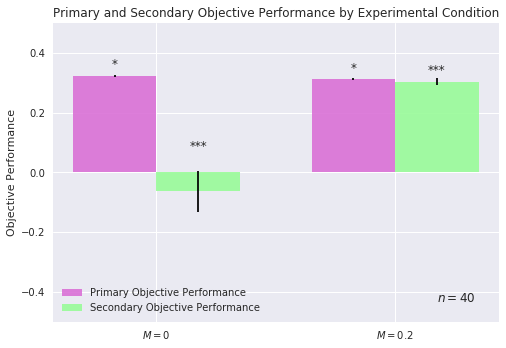
\includegraphics[width=0.8\textwidth]{img/primary_secondary_performance}
 	\captionsetup{singlelinecheck=off,justification=raggedright}
  	\caption{Comparison of objective performances of champions evolved with only primary condition/objective pair versus with both primary and secondary condition/objective pairs.}
    \label{fig:ev_w0}
\end{figure}
\end{frame}

\begin{frame}{Generating and Reading an Evolvability Signature}
  \begin{figure}
  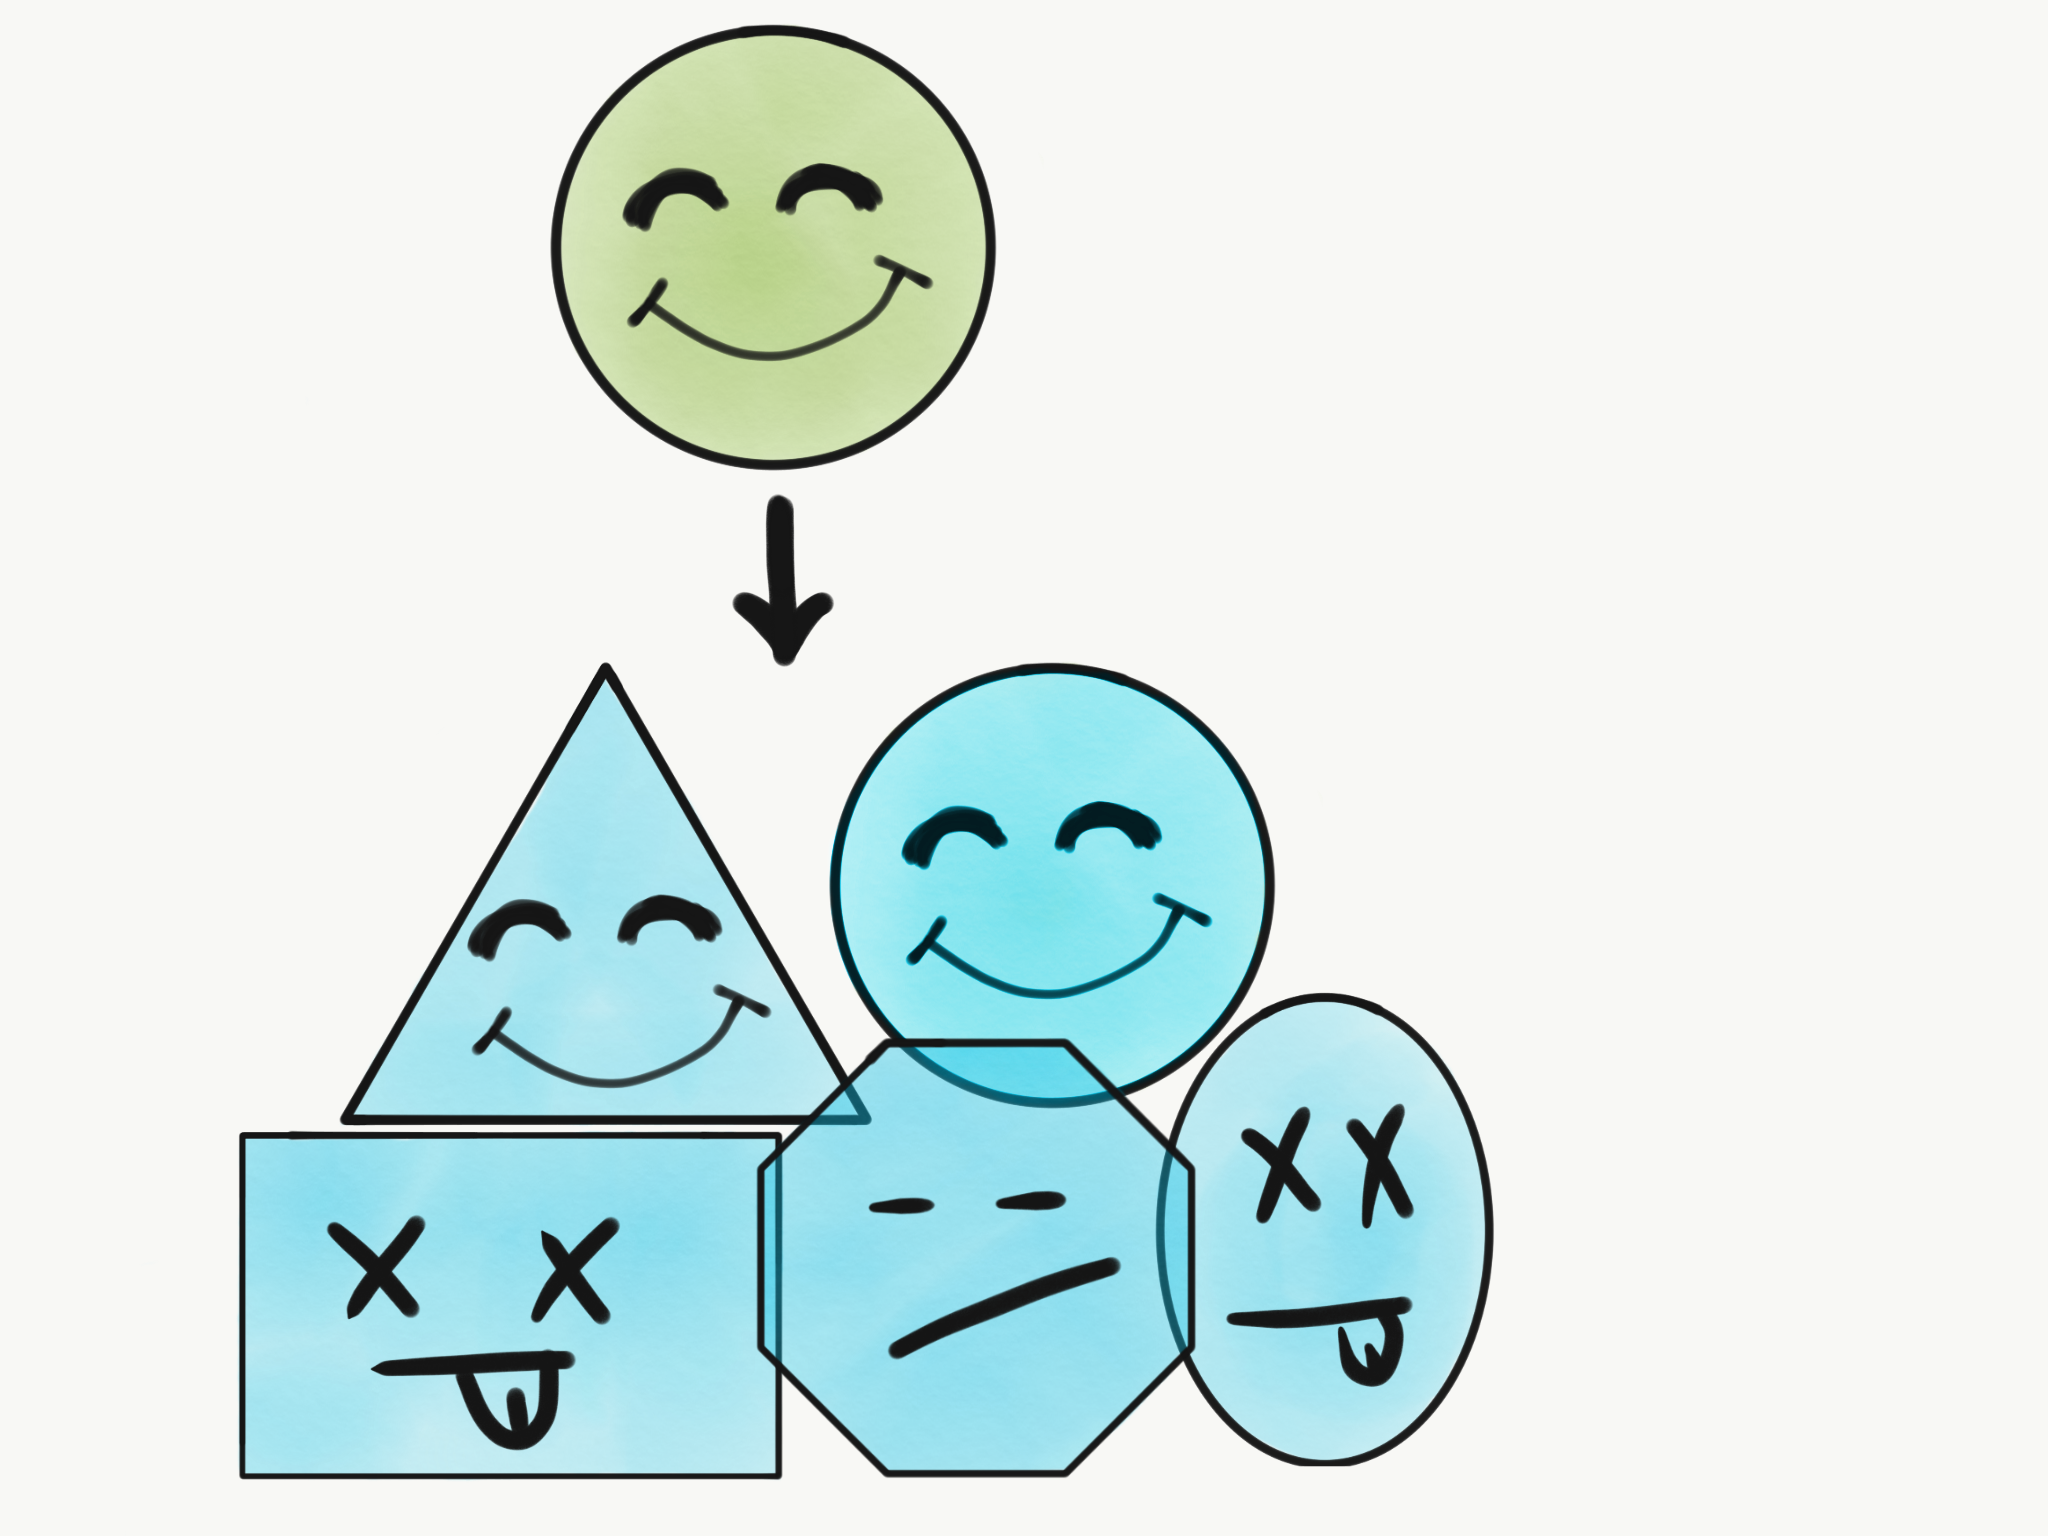
\includegraphics[width=0.5\textwidth]{img/evol_sig_gen}
  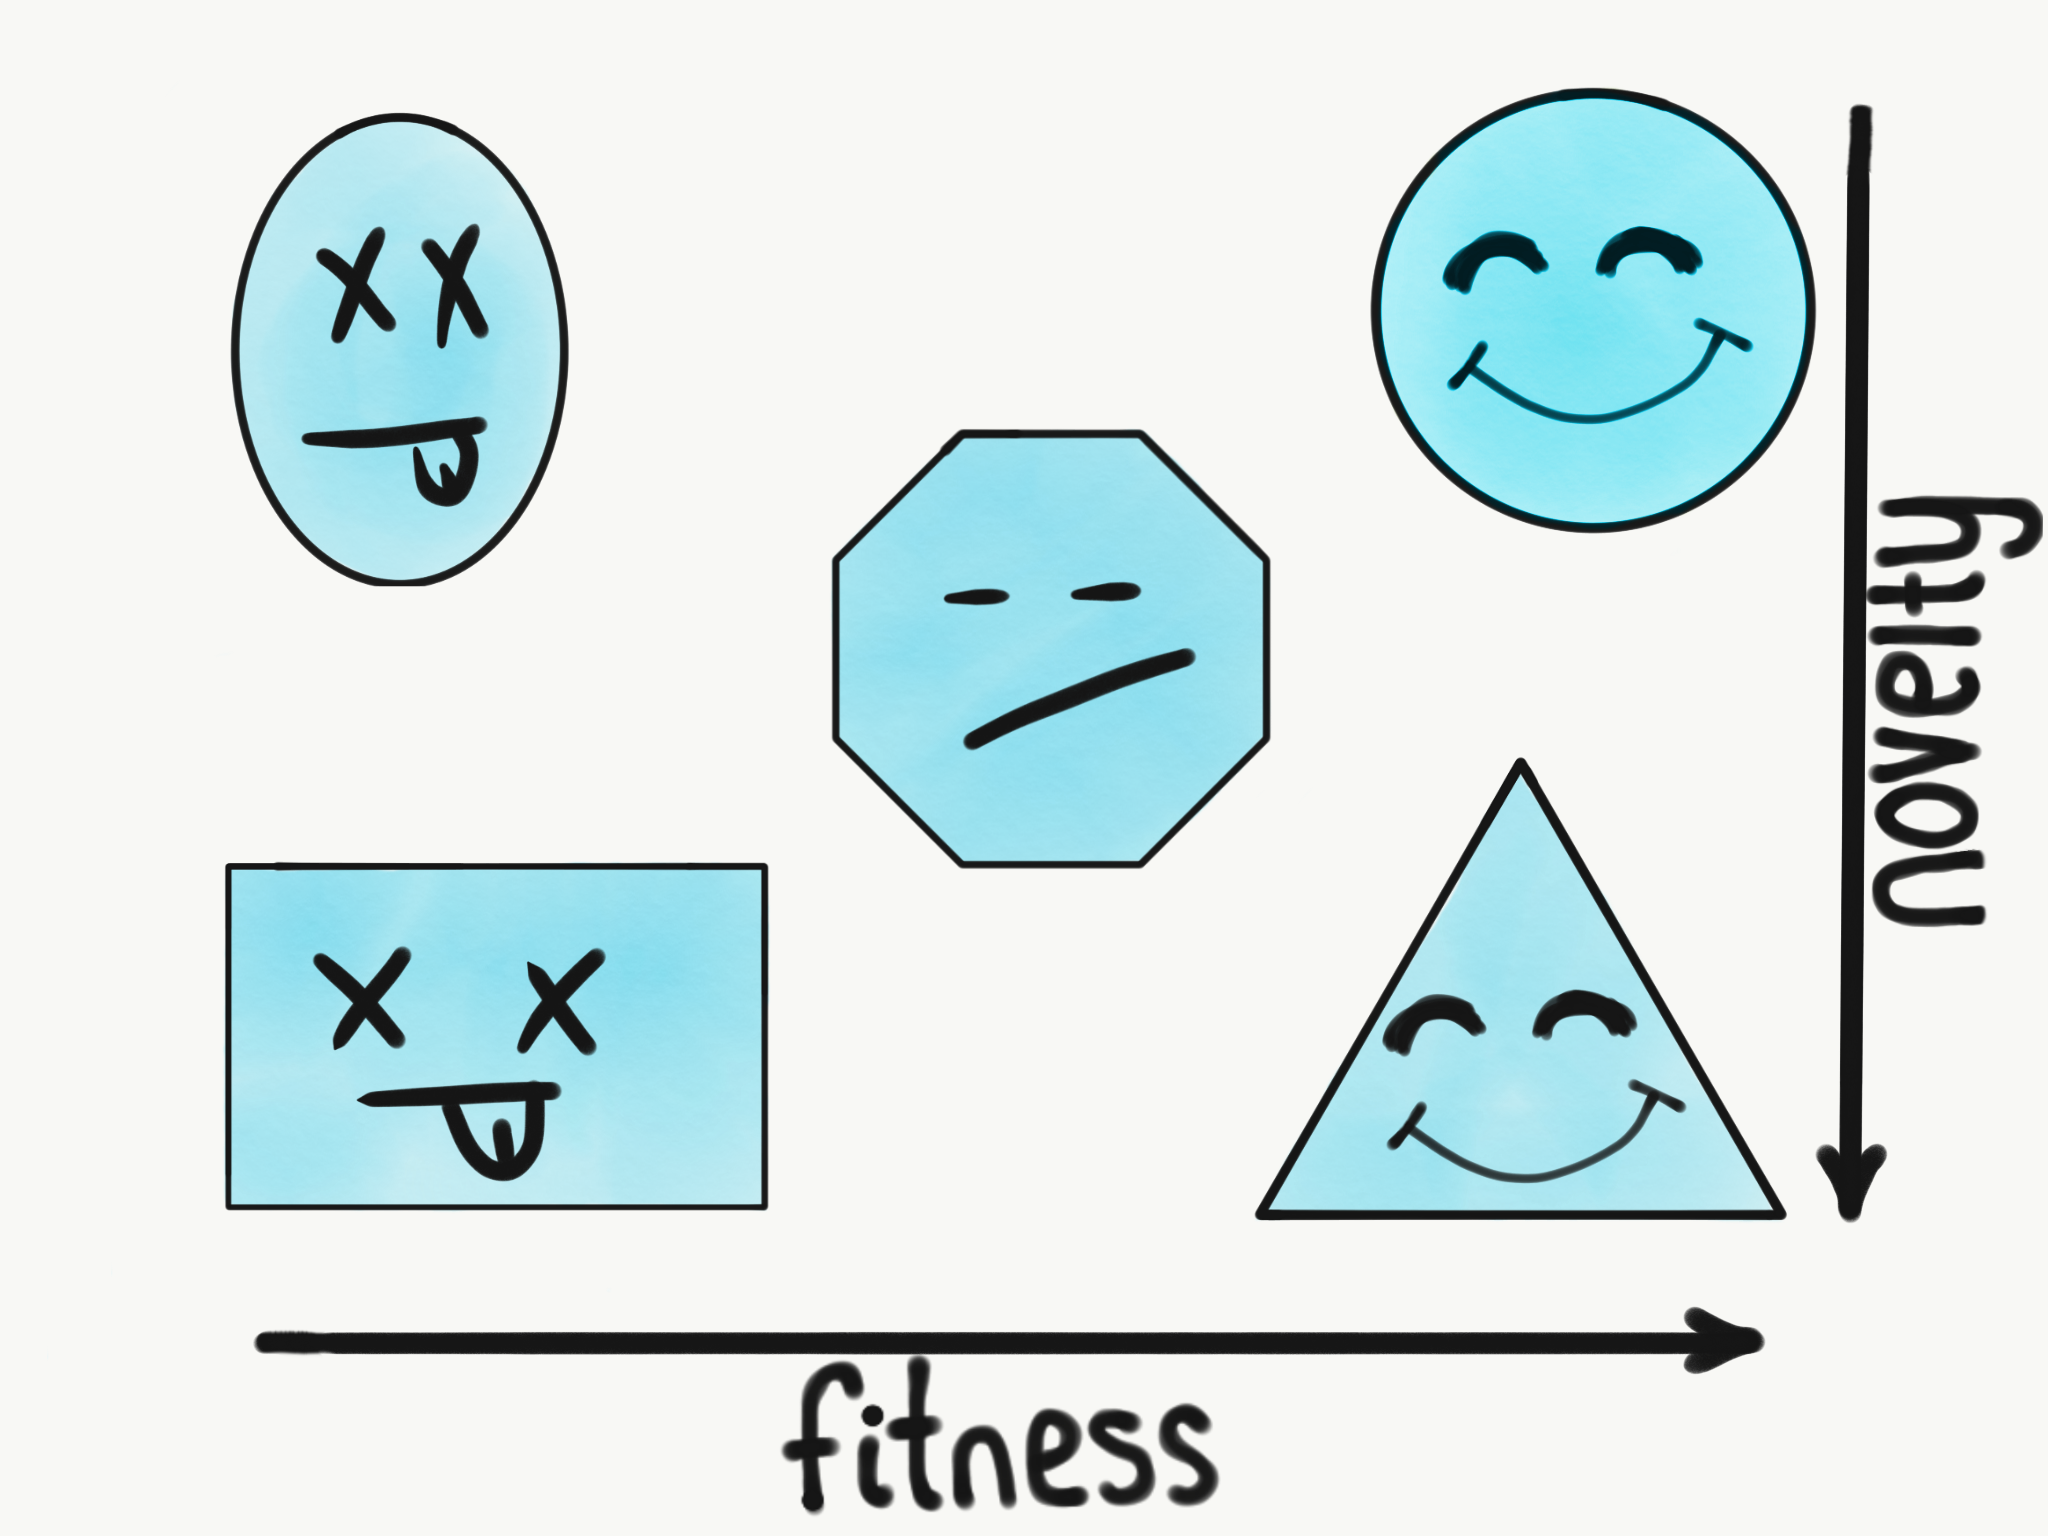
\includegraphics[width=0.5\textwidth]{img/evol_sig_read}
  \captionsetup{singlelinecheck=off,justification=raggedright}
  \caption{Cartoon illustration describing the creation and layout of an evolvability signature diagram \cite{Tarapore2015EvolvabilityBenchmarks}.}
  \label{fig:reading_evolvability_signature}
\end{figure}
\end{frame}

\begin{frame}{Evolvability Visualization $W=0$} 
\begin{figure}
    \centering
    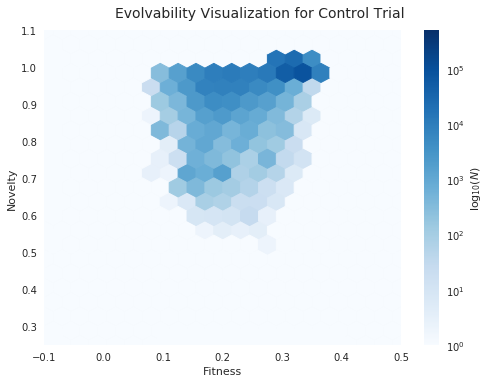
\includegraphics[width=0.8\textwidth]{img/ev_w0}
 	\captionsetup{singlelinecheck=off,justification=raggedright}
  	\caption{Evolvability visualization of champions evolved with only a primary condition/objective pair.}
    \label{fig:ev_w0}
\end{figure}
\end{frame}

\begin{frame}{Evolvability Visualization $W=0.2$}
\begin{figure}
    \centering
    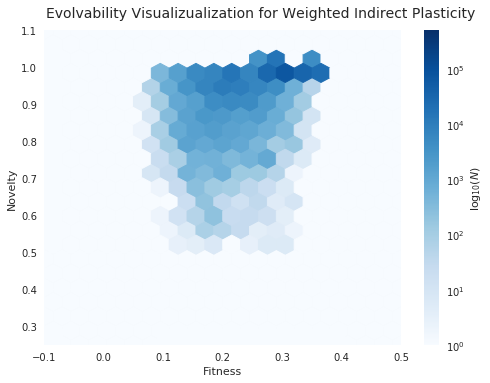
\includegraphics[width=0.8\textwidth]{img/ev_w0_2}
 	\captionsetup{singlelinecheck=off,justification=raggedright}
  	\caption{Evolvability visualization of champions evolved with primary and secondary condition/objective pairs.}
    \label{fig:es_w0_2}
\end{figure}
\end{frame}


\begin{frame}{Environmental Influence on the Phenotype}
\begin{itemize}
	\item in biology, genotype not sole determinant of phenotype
    \item $P = G + E$
    \item plasticity: phenotypic response to the environment
    \item direct plasticity versus indirect plasticity
\end{itemize}
\end{frame}

\begin{frame}{Direct Plasticity: Biological Intuition}
  \begin{figure} \label{fig:elephant_developmental_perturbation}
  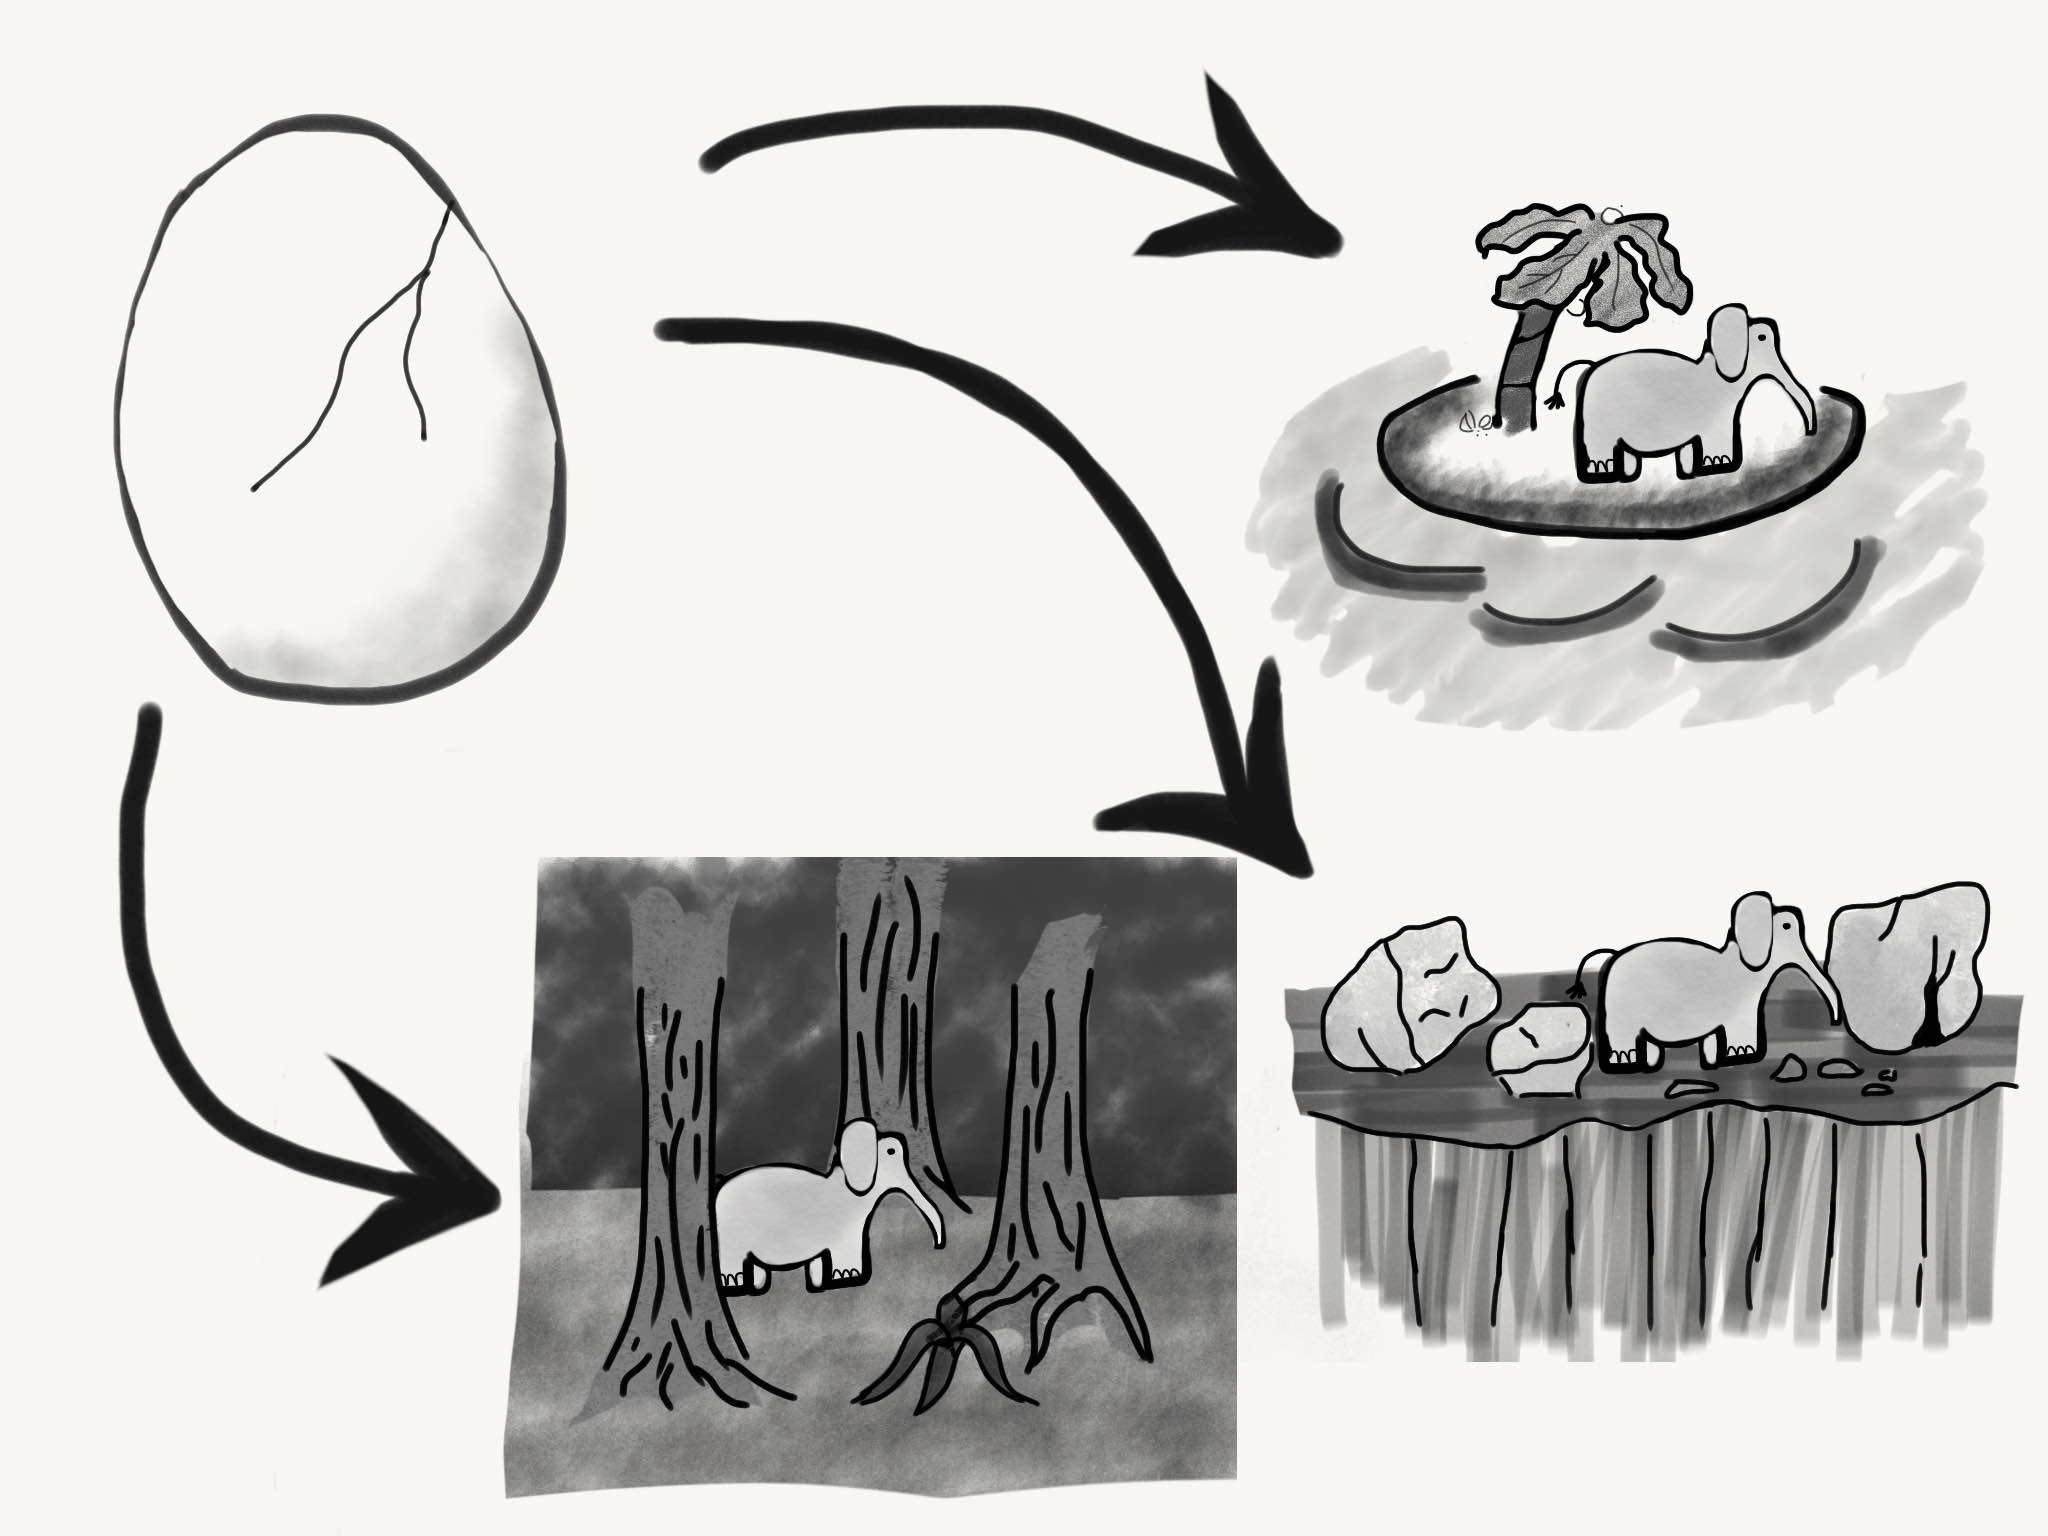
\includegraphics[width=0.8\textwidth]{img/elephant_developmental_perturbation.jpg}
  \captionsetup{singlelinecheck=off,justification=raggedright}

  \caption{A cartoon illustration of resistance to environmental perturbation.}
\end{figure}
\end{frame}

\begin{frame}{Indirect Plasticity: Biological Intuition}
  \begin{figure} \label{figs/plant_developmental_perturbation}
  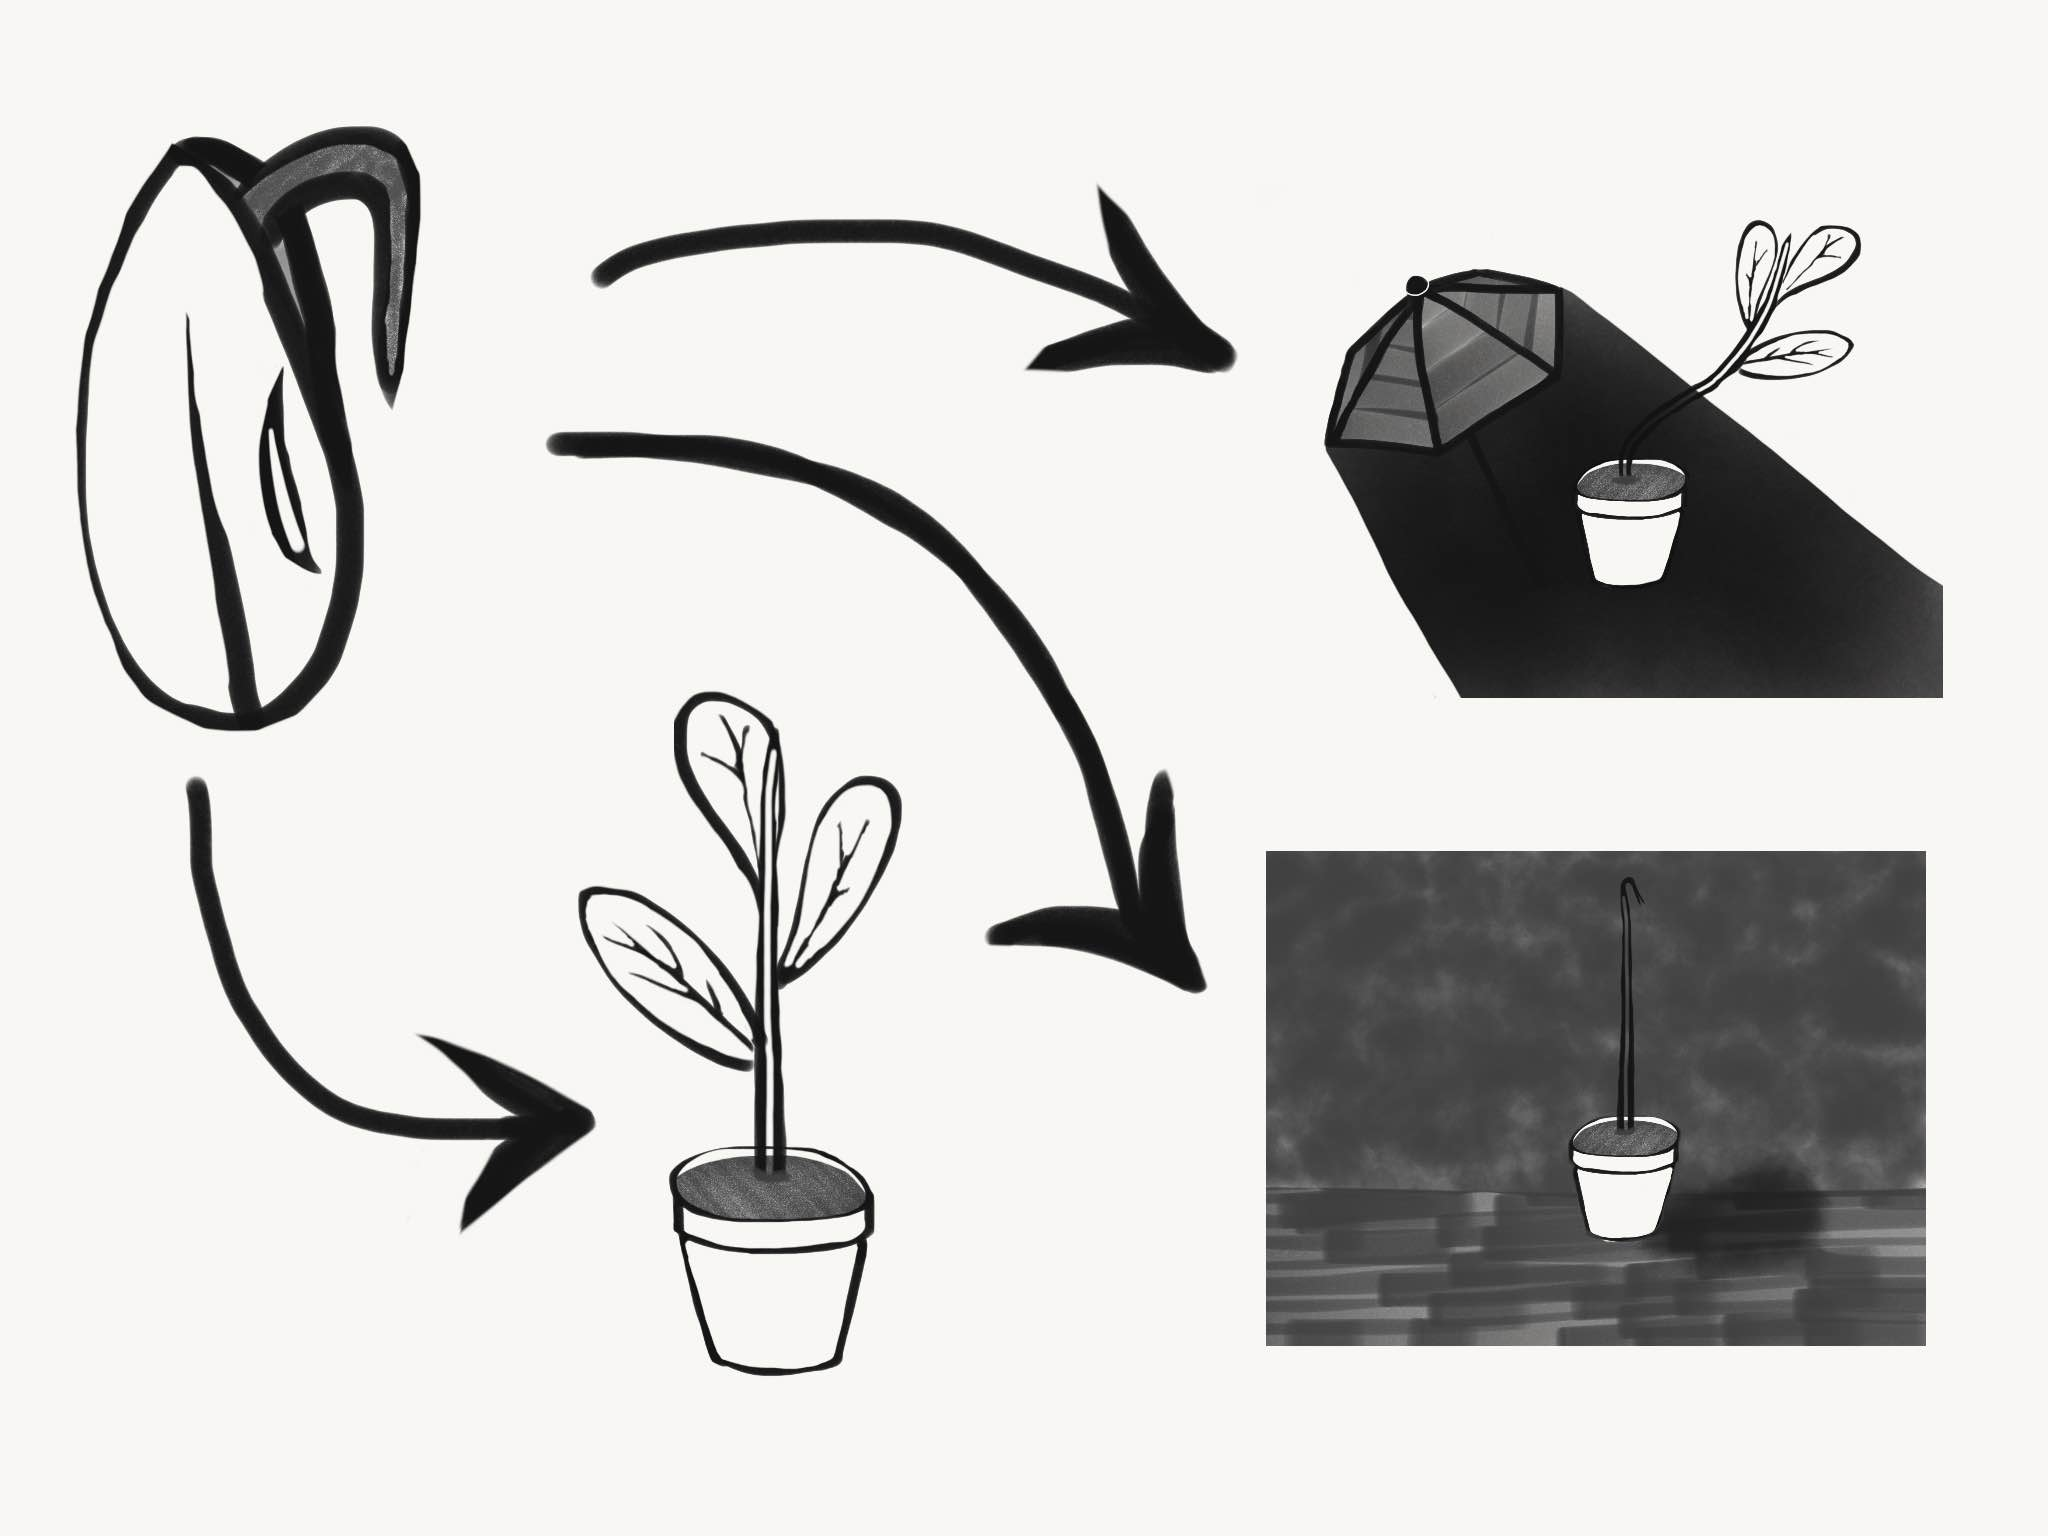
\includegraphics[width=0.8\textwidth]{img/plant_developmental_perturbation.jpg}
  \captionsetup{singlelinecheck=off,justification=raggedright}
  \caption{A cartoon illustration of alternate phenotypes expressed based on environmental signals.}
\end{figure}

\end{frame}

\begin{frame}{Complete Model}
\begin{figure}
    \centering
    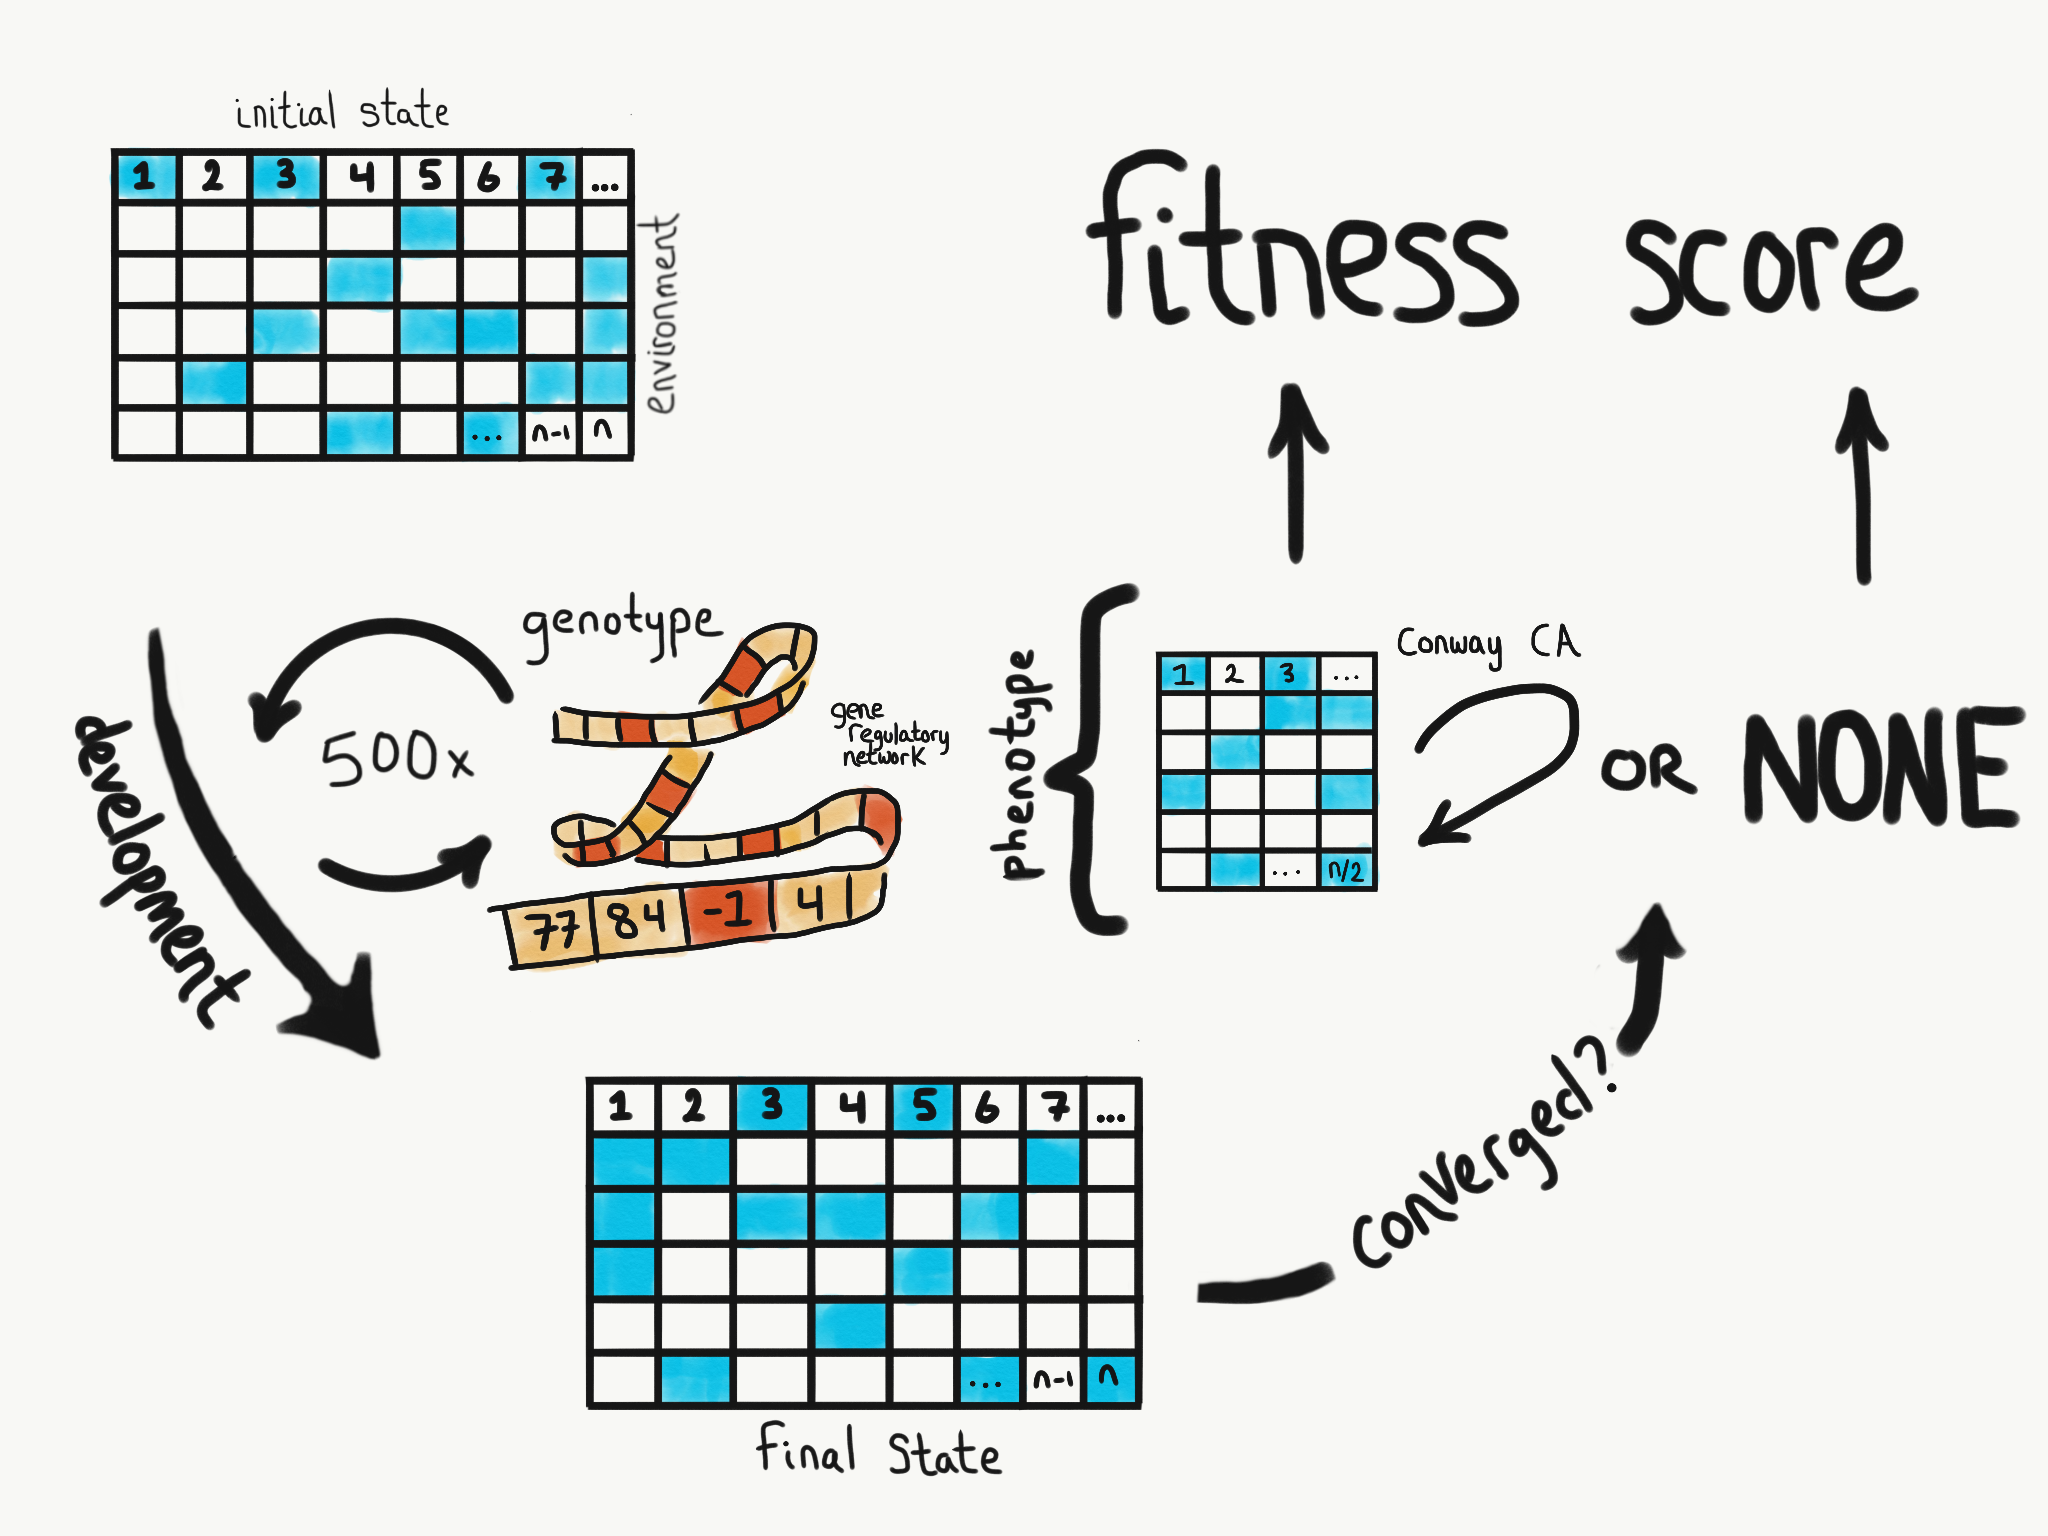
\includegraphics[width=0.8\textwidth]{img/complete_schematic}
 	\captionsetup{singlelinecheck=off,justification=raggedright}
  	\caption{A cartoon overview of the development and assessment processes of the expanded model, based loosely on \cite{Wilder2015ReconcilingEvolvability}.}
    \label{fig:complete_schematic}
\end{figure}
\end{frame}

\begin{frame}{Biological Perspective: Intraindividual Degeneracy}
  idea: employing a diverse collection of substructures that provide identical or near-identical functionality promote robustness through redundancy while providing many jumping off points for variation through repurposing or elaboration
  \begin{figure}
 \begin{columns}
 \begin{column}{0.6\textwidth}
 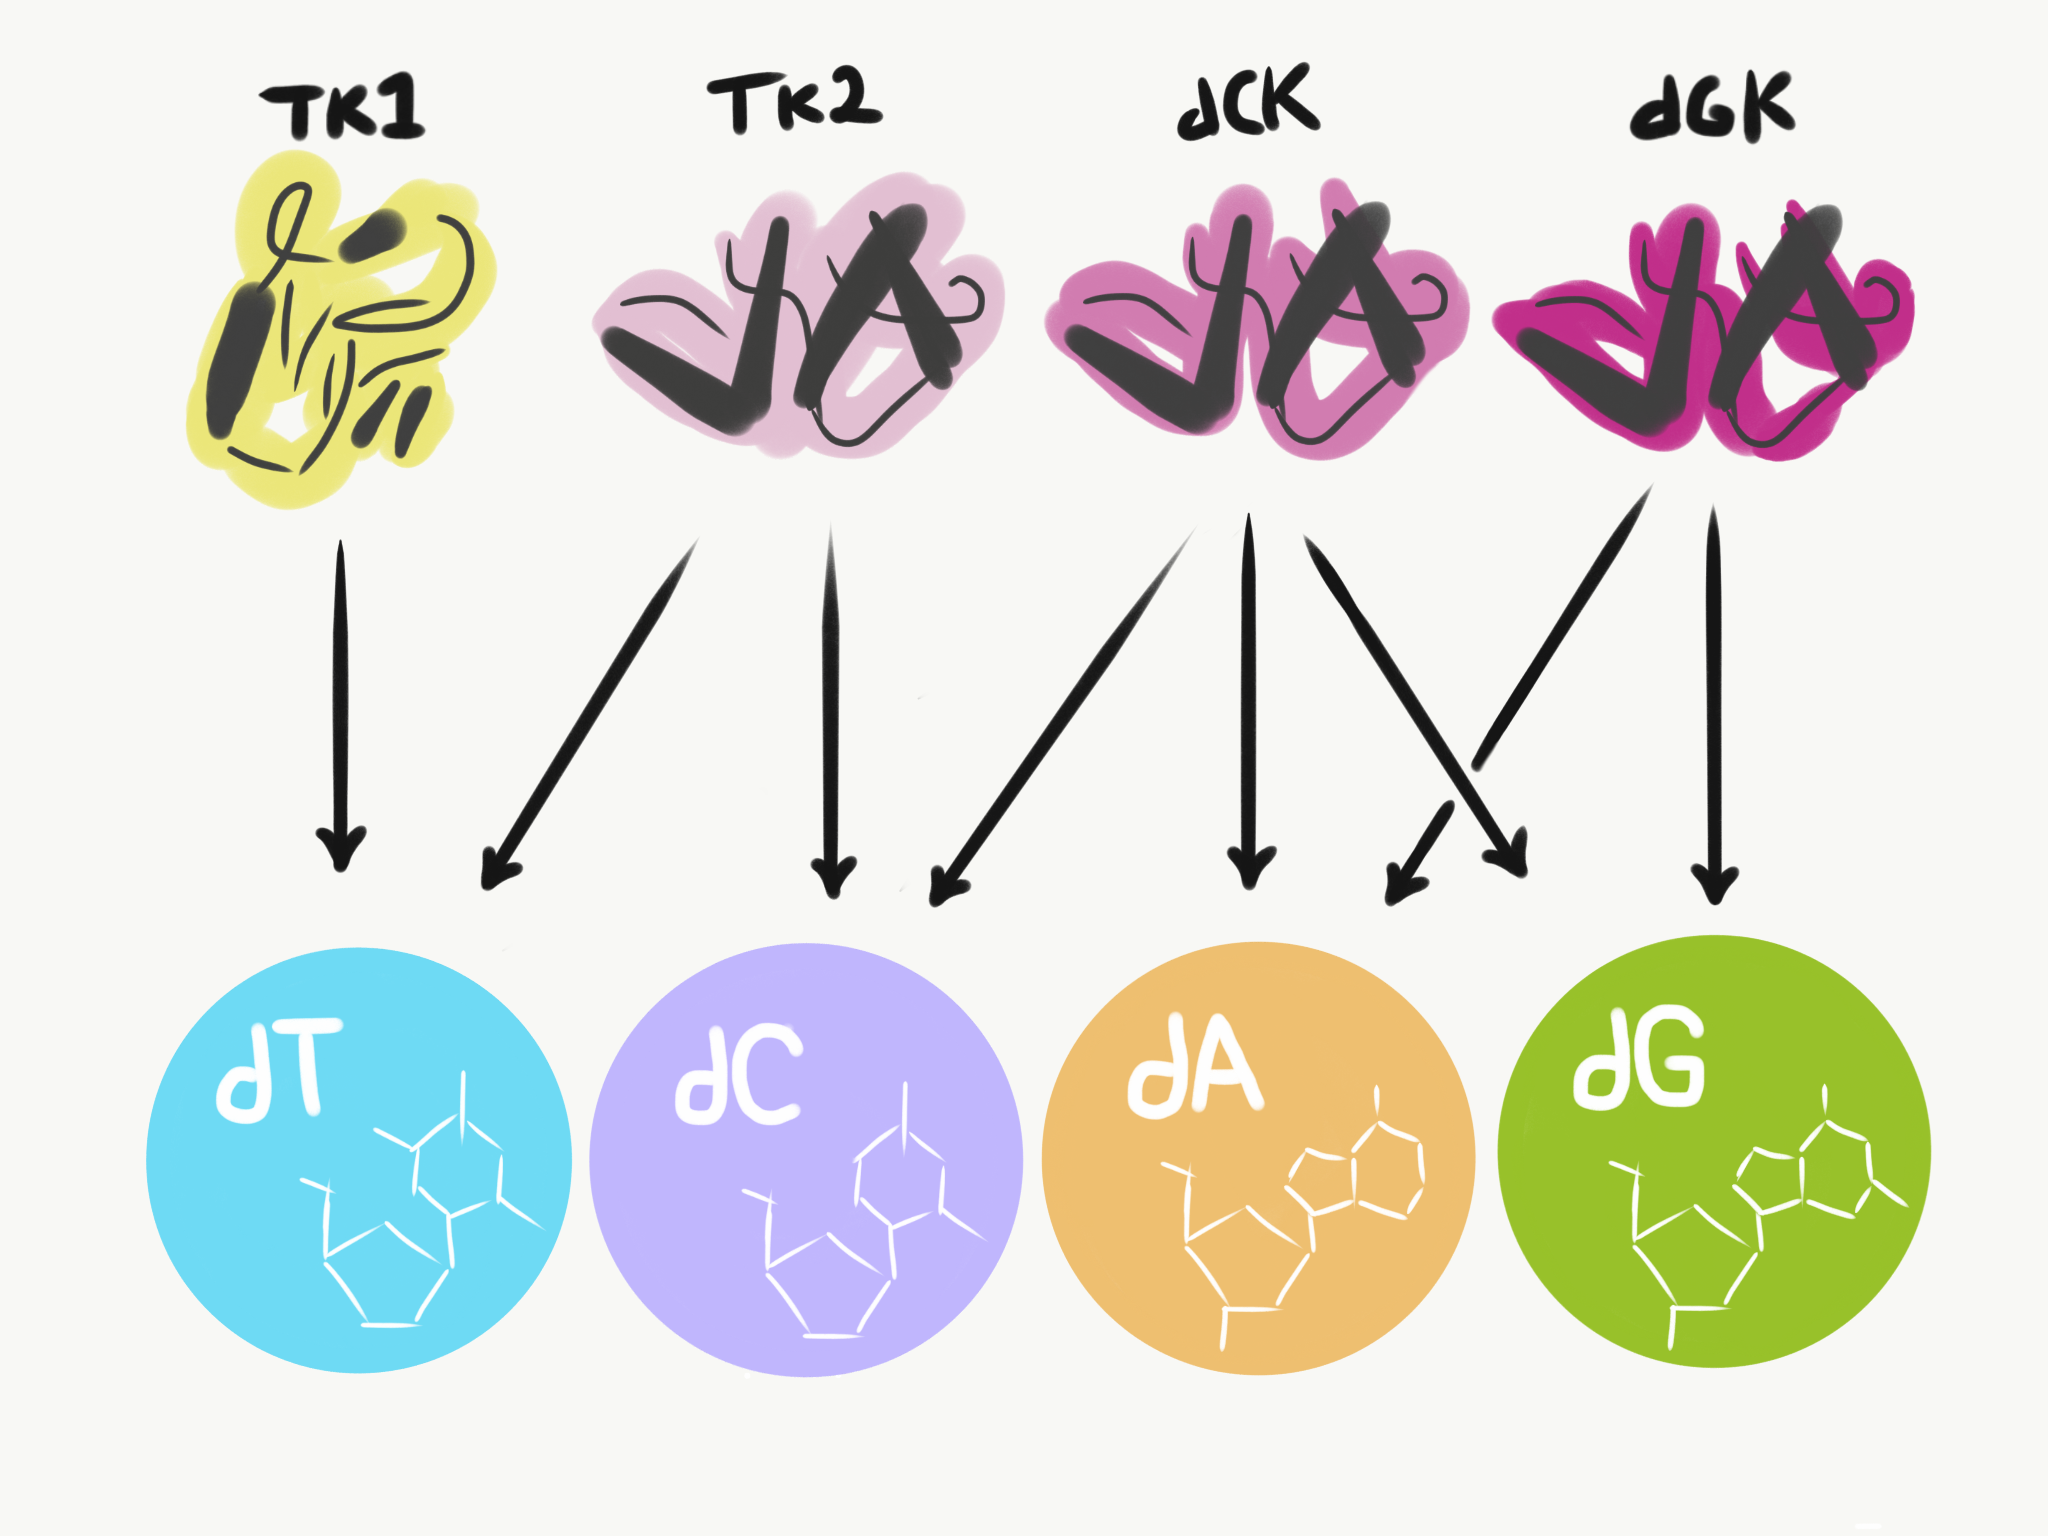
\includegraphics[width=\textwidth]{img/intraindividual_degeneracy}
 \end{column}
 \begin{column}{0.4\textwidth}
\captionsetup{singlelinecheck=off,justification=raggedright}
  	\caption{Mammalian deoxyribonucleoside kinases exhibit degeneracy \cite{Sandrini2005DeoxyribonucleosideReaction.}.}
    \label{fig:intraindividual_degeneracy}
    
\end{column}
\end{columns}
\end{figure}
\end{frame}

\begin{frame}{Conway's Game of Life}
\begin{figure}
  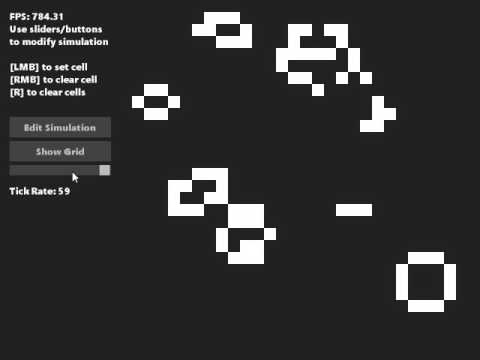
\includegraphics[width=0.8\textwidth]{img/gol_icon}
  \captionsetup{singlelinecheck=off,justification=raggedright}
\href{https://www.youtube.com/watch?v=Kzg5is1lgSk}{\caption{Video illustrations of Conway's Game of Life cellular automata in action.}}
\end{figure}
\end{frame}

\begin{frame}{Evidence for Indirect Plasticity}
\begin{figure}
    \centering
    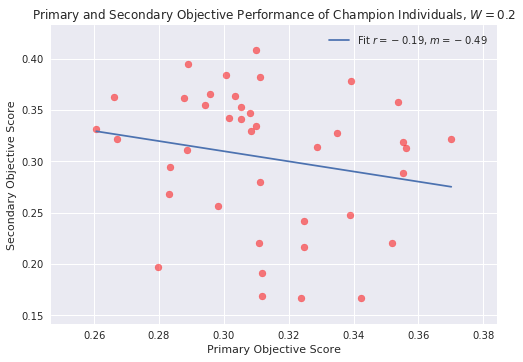
\includegraphics[width=0.8\textwidth]{img/primary_secondary_w02}
 	\captionsetup{singlelinecheck=off,justification=raggedright}
  	\caption{Primary and secondary objective performance of champion individuals evolved with primary and secondary condition/objective pair.}
    \label{fig:ev_w0}
\end{figure}
\end{frame}

\begin{frame}{Evidence for Indirect Plasticity}
\begin{figure}
    \centering
    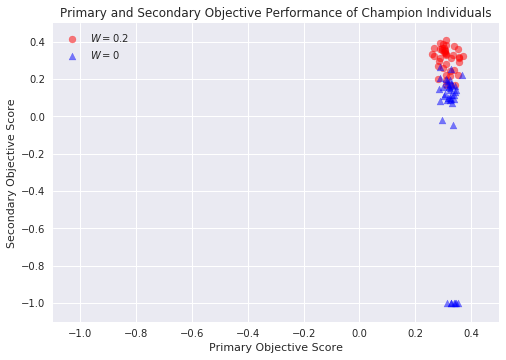
\includegraphics[width=0.8\textwidth]{img/scatter_indirect}
 	\captionsetup{singlelinecheck=off,justification=raggedright}
  	\caption{Comparison of objective performances of champions evolved with only primary condition/objective pair versus with both primary and secondary condition/objective pairs.}
    \label{fig:es_p0}
\end{figure}
\end{frame}

\begin{frame}{Evolvability as Novel Variation}
  \begin{figure}
 \centering
    \begin{subfigure}[b]{0.5\textwidth}
        \centering
    	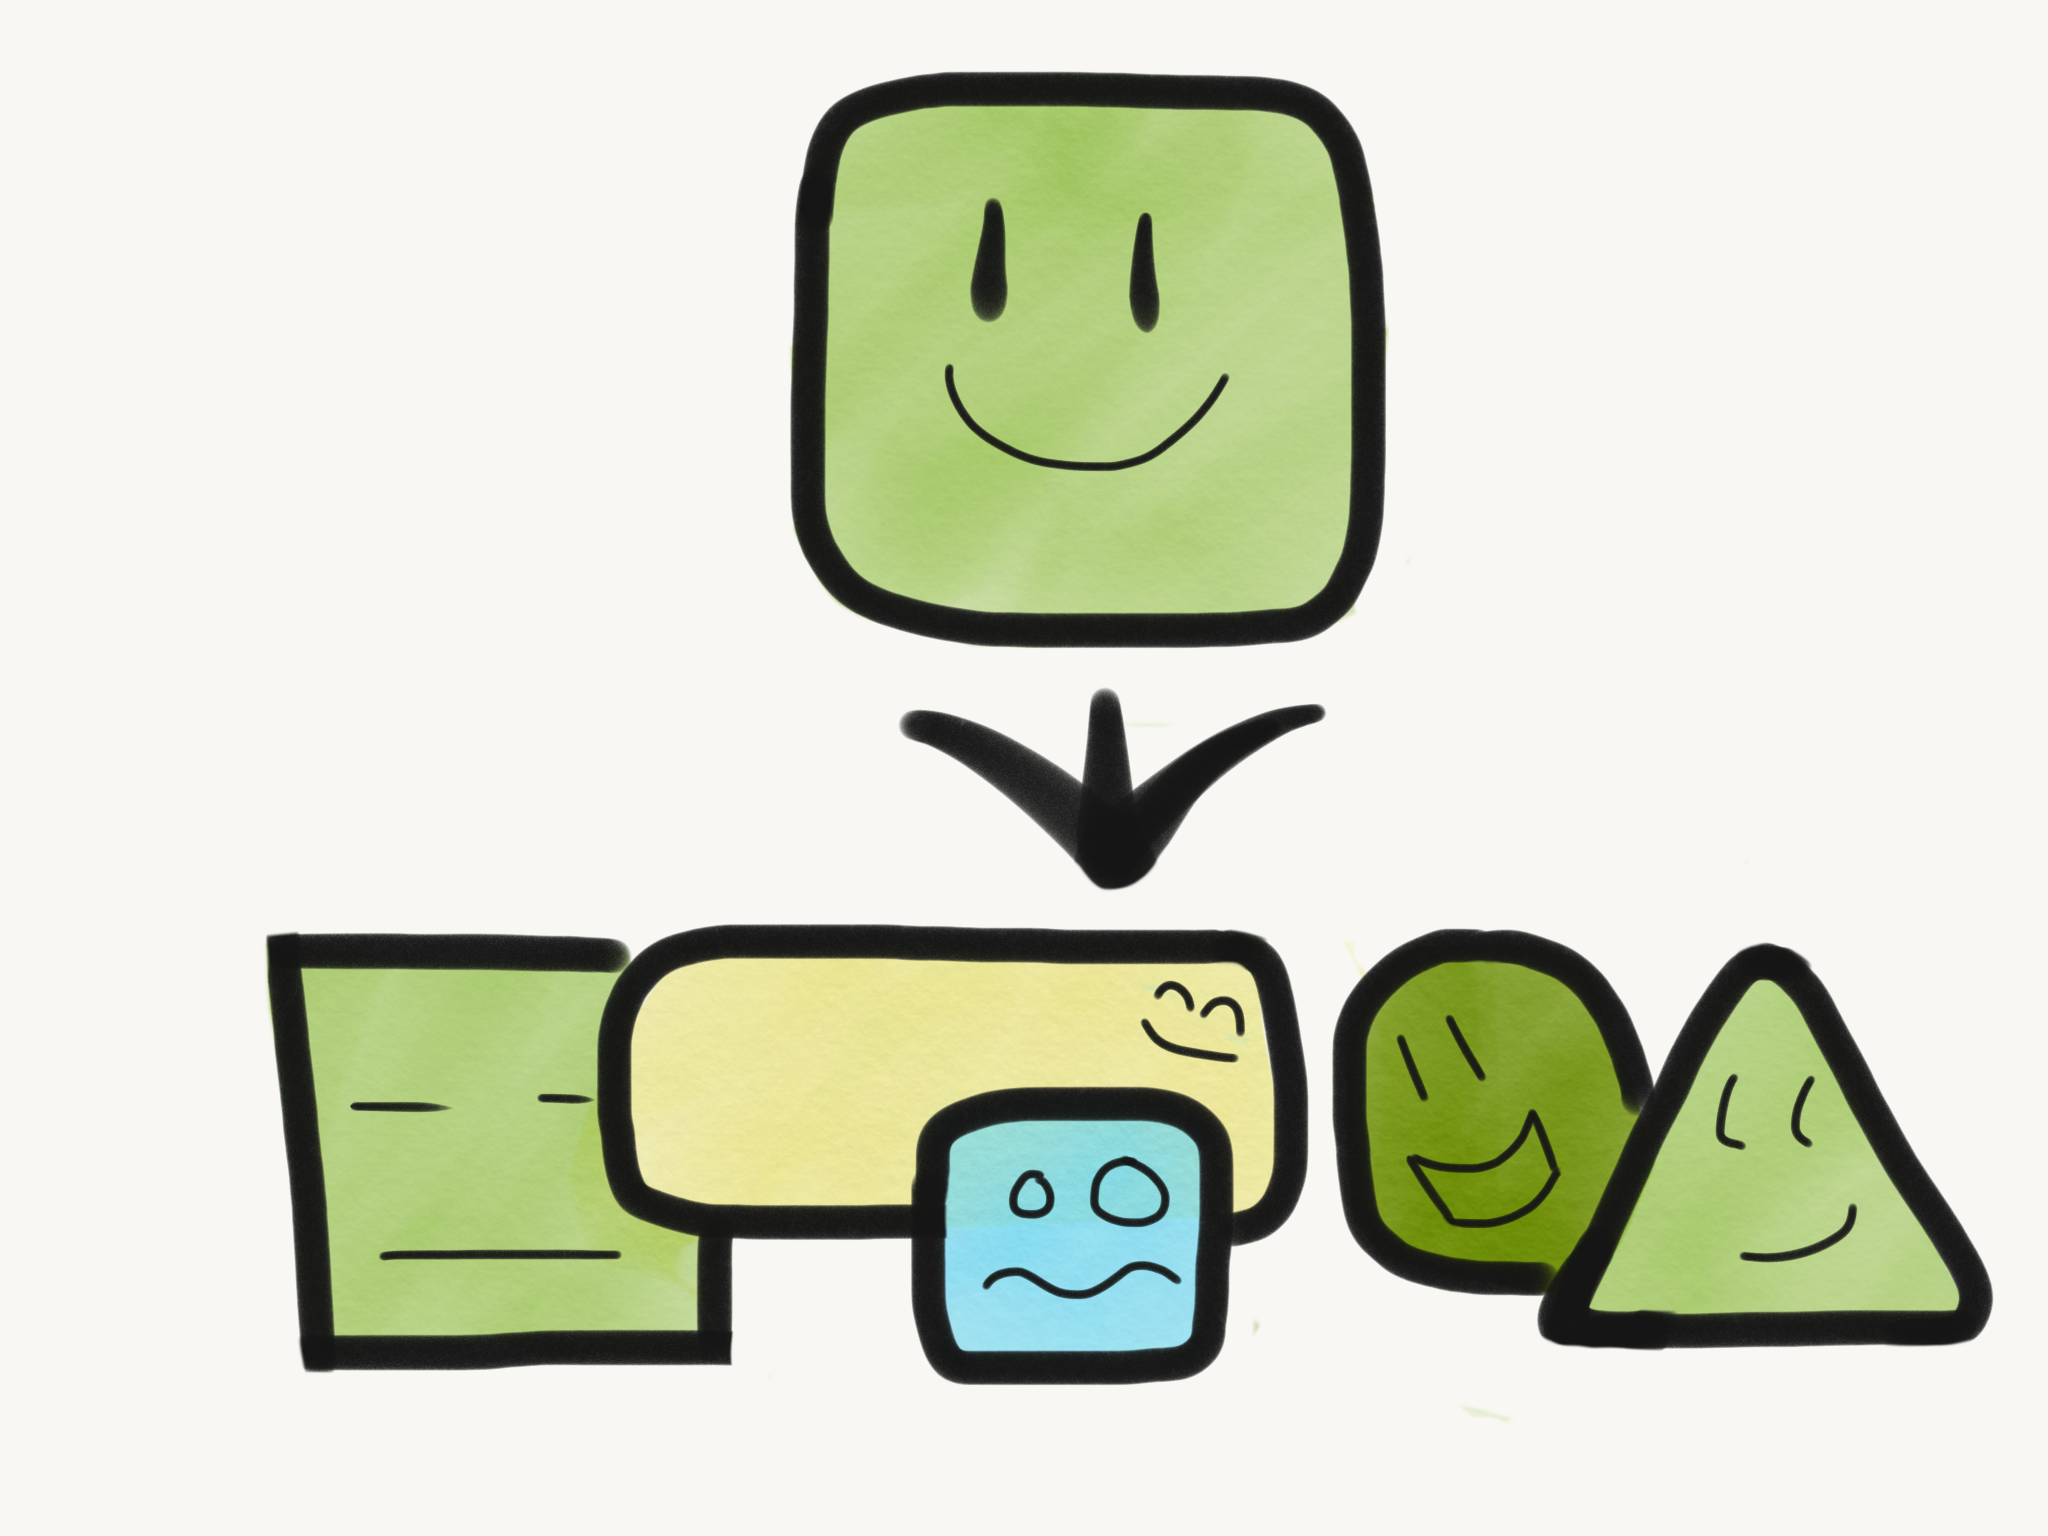
\includegraphics[width=\textwidth]{img/individual_evolvability}
        \caption{individual evolvability}
        \label{subfig:individual_evolvability}
    \end{subfigure}%
    \hfill
    \begin{subfigure}[b]{0.5\textwidth}
        \centering
        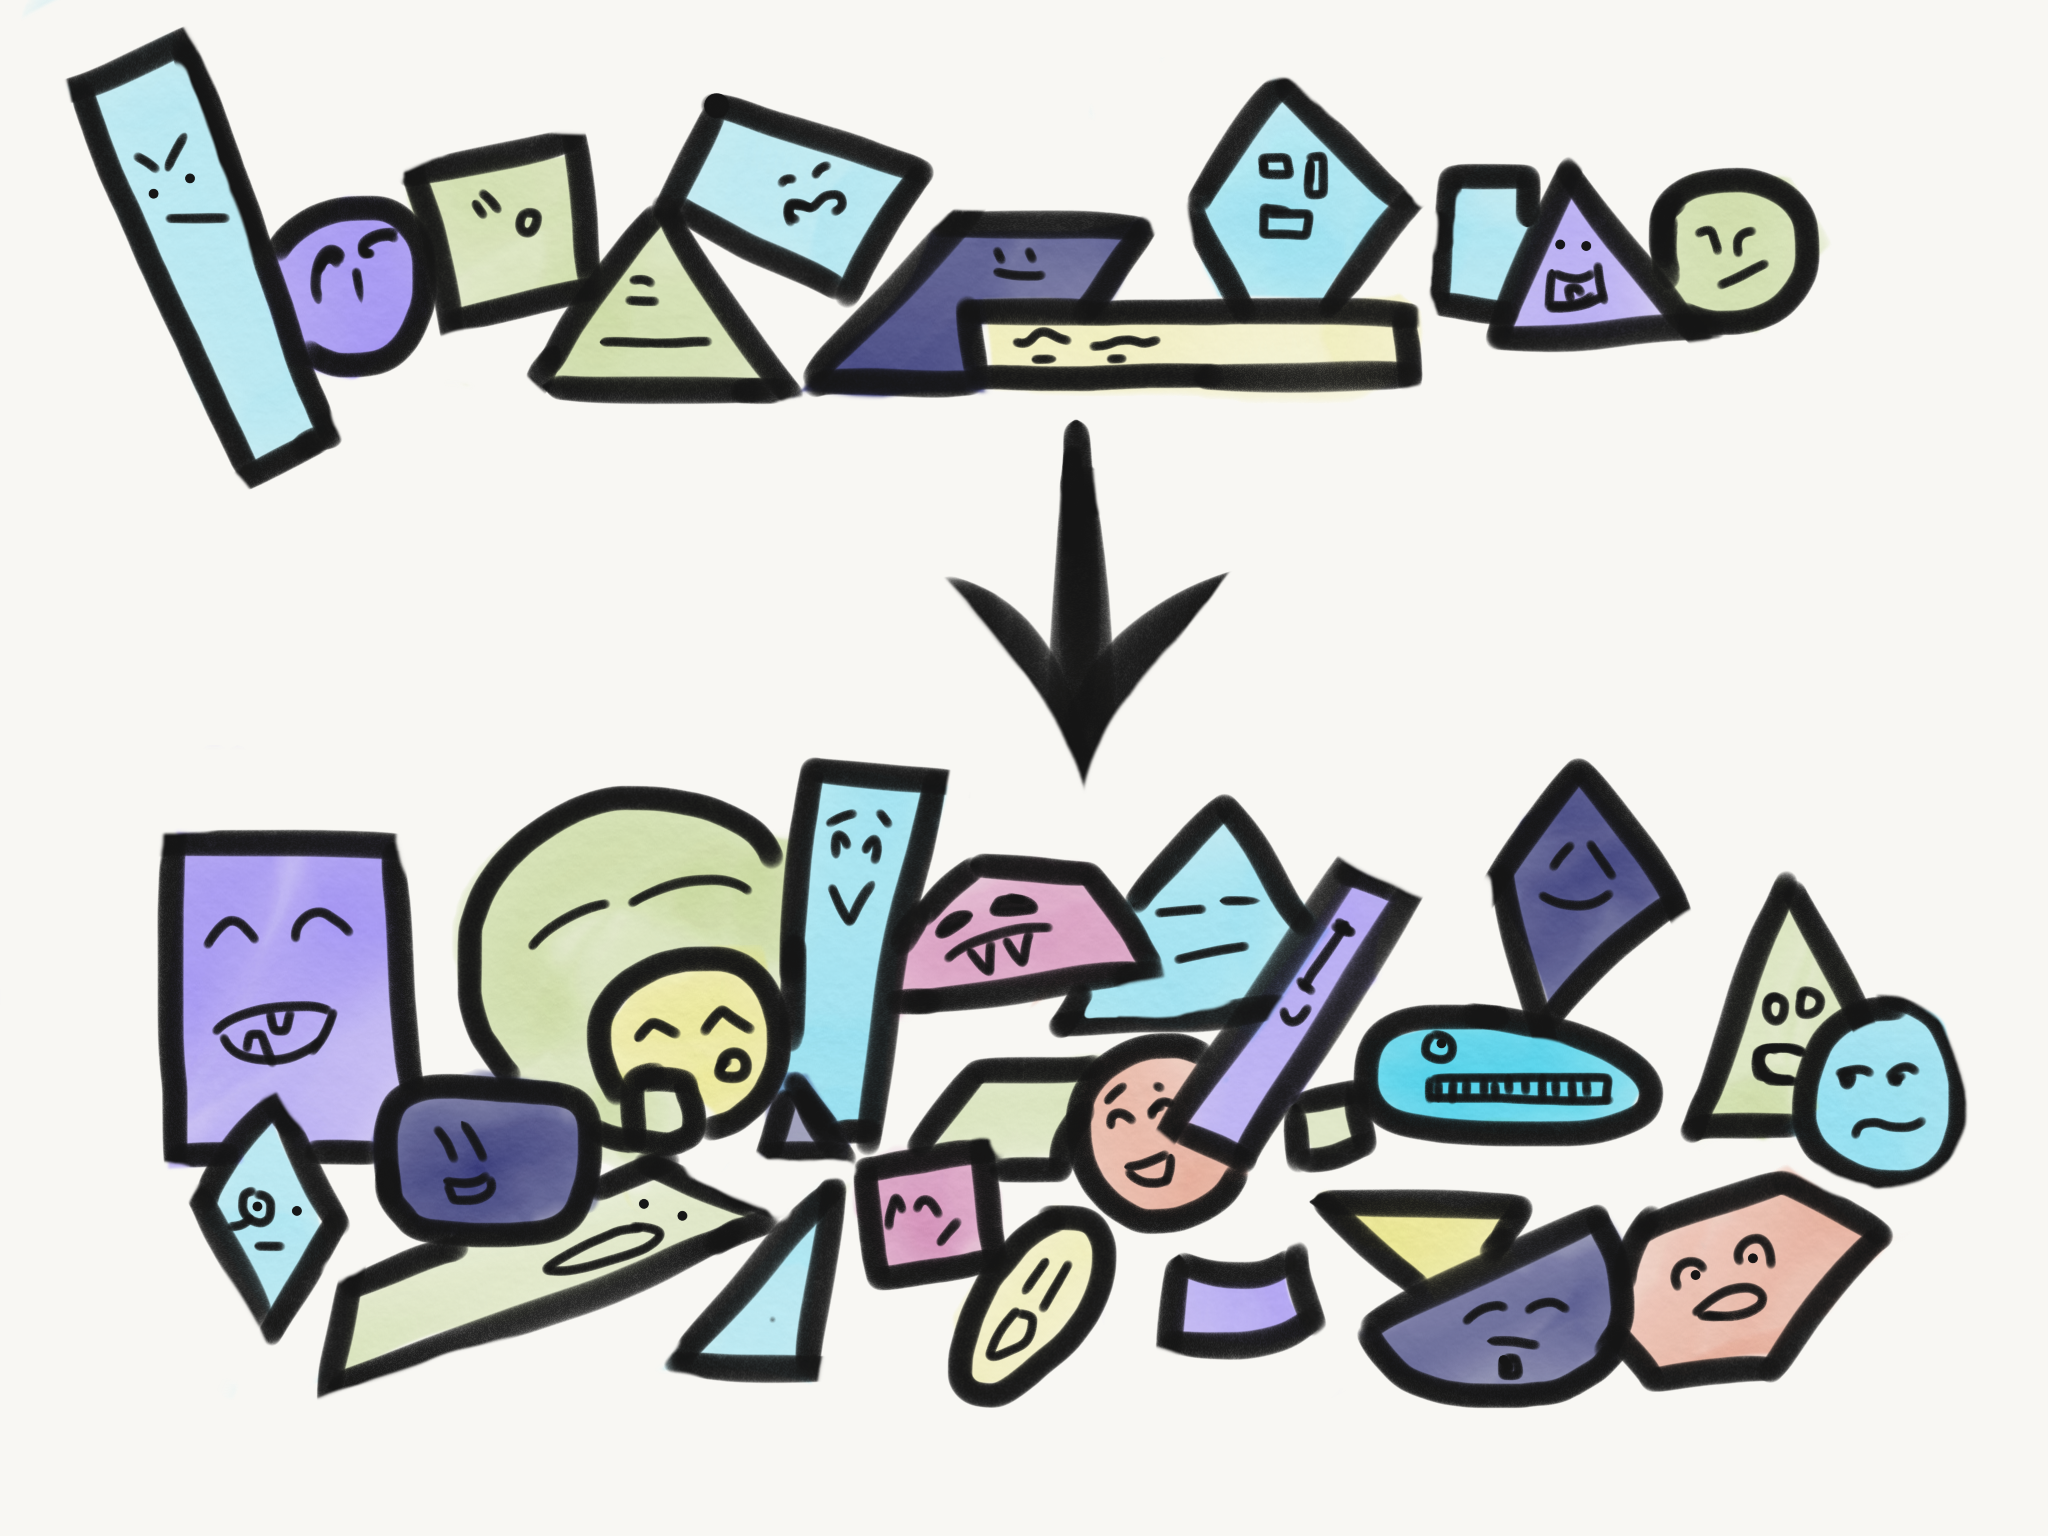
\includegraphics[width=\textwidth]{img/population_evolvability}
        \caption{population evolvability}
        \label{subfig:population_evolvability}
    \end{subfigure}
 	\captionsetup{singlelinecheck=off,justification=raggedright}
    \vspace{-4ex}
  \captionsetup{singlelinecheck=off,justification=raggedright}
  \caption{An illustration contrasting individual and population evolvability \cite{Wilder2015ReconcilingEvolvability}.}
  \label{fig:individual_vs_population_evolvability}
\end{figure}
\end{frame}

\begin{frame}{Promoting Evolvability: Fitness Niches}
	\begin{figure}
\begin{center}
\label{fig:cppn_images}
  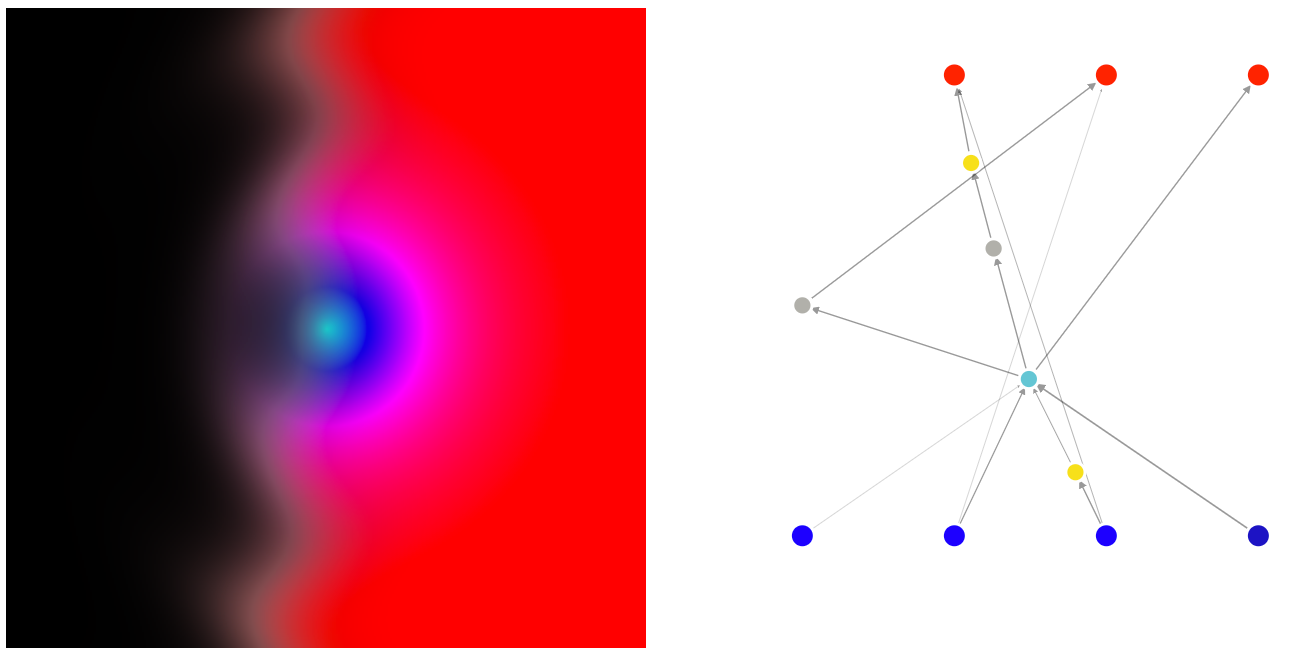
\includegraphics[width=0.4\textwidth]{img/parent} \\
  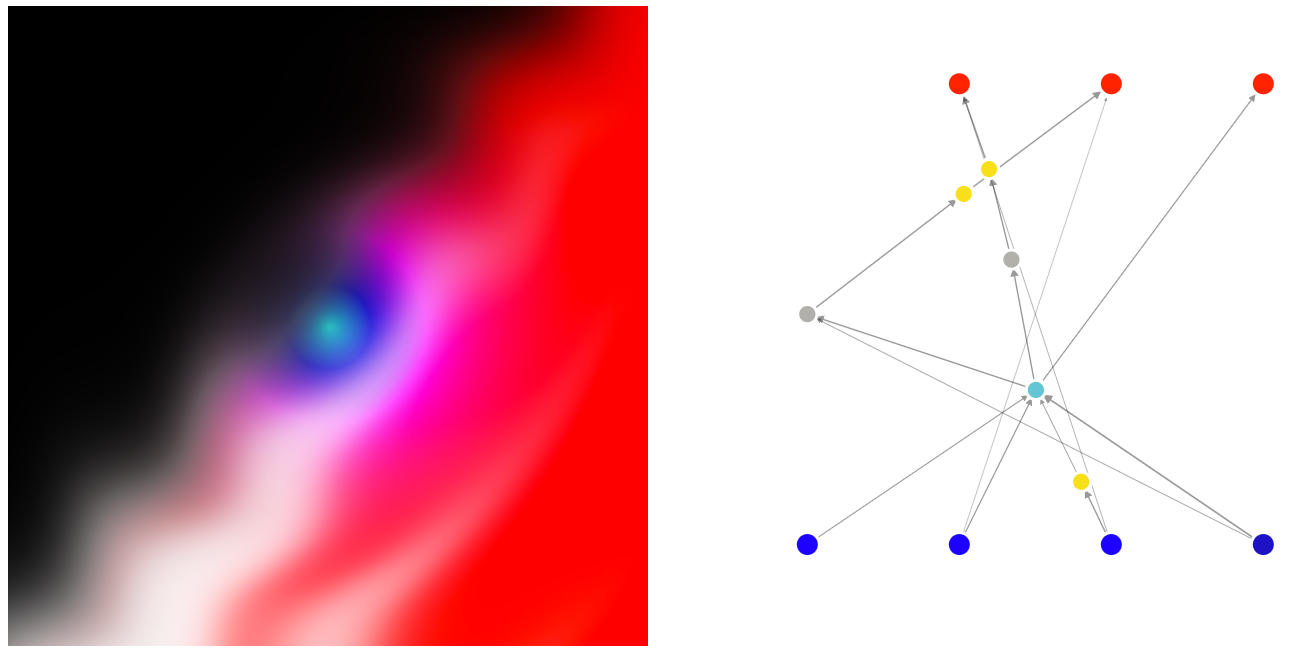
\includegraphics[width=0.4\textwidth]{img/offspring} \\
  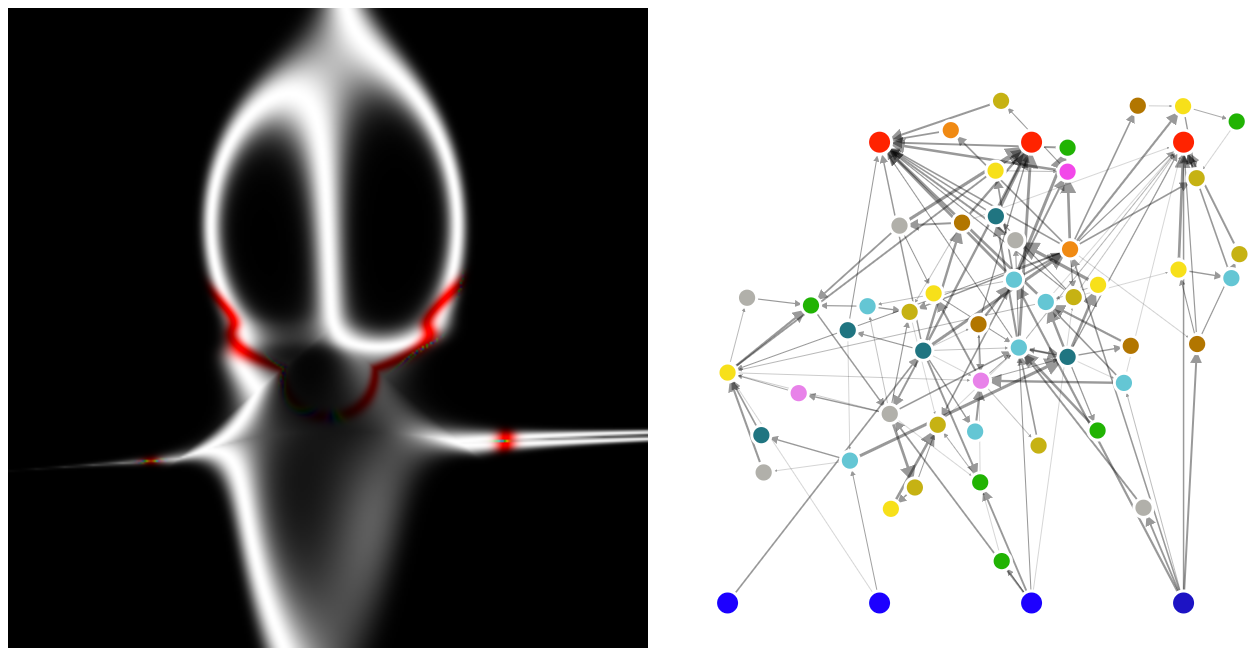
\includegraphics[width=0.4\textwidth]{img/better_goast}
  \end{center}
  \captionsetup{singlelinecheck=off,justification=raggedright}

  \caption{Illustration of compositional pattern producing networks (right) and their output images (left) generated via \cite{Ha2015Neurogram}.}
\end{figure}
\end{frame}

\begin{frame}{Promoting Evolvability: Fitness Niches}
\vfill
	\begin{figure} \label{fig:dnn}
  \begin{center}
  
\includegraphics[width=0.5\textwidth]{img/recognize} \\
  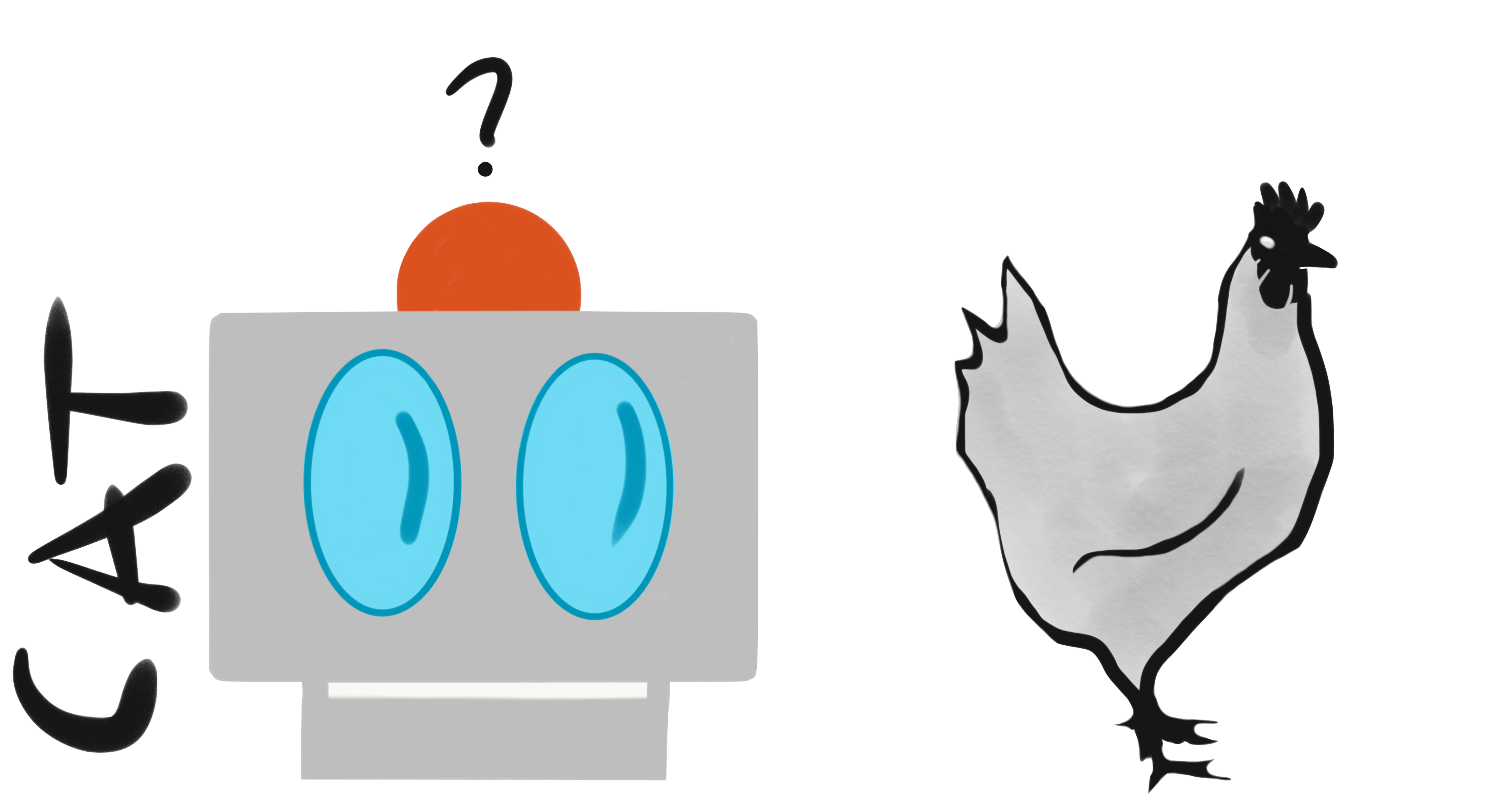
\includegraphics[width=0.5\textwidth]{img/confused}
  \end{center}
  \captionsetup{singlelinecheck=off,justification=raggedright}

  \caption{A deep neural network (DNN) is trained to recognize a specific category of images.}
\end{figure}
    \vfill
\end{frame}

\begin{frame}{Promoting Evolvability: Fitness Niches}
\vspace{2ex}
	\begin{figure}
    \centering
  \begin{columns}
  \begin{column}{0.6\textwidth}
  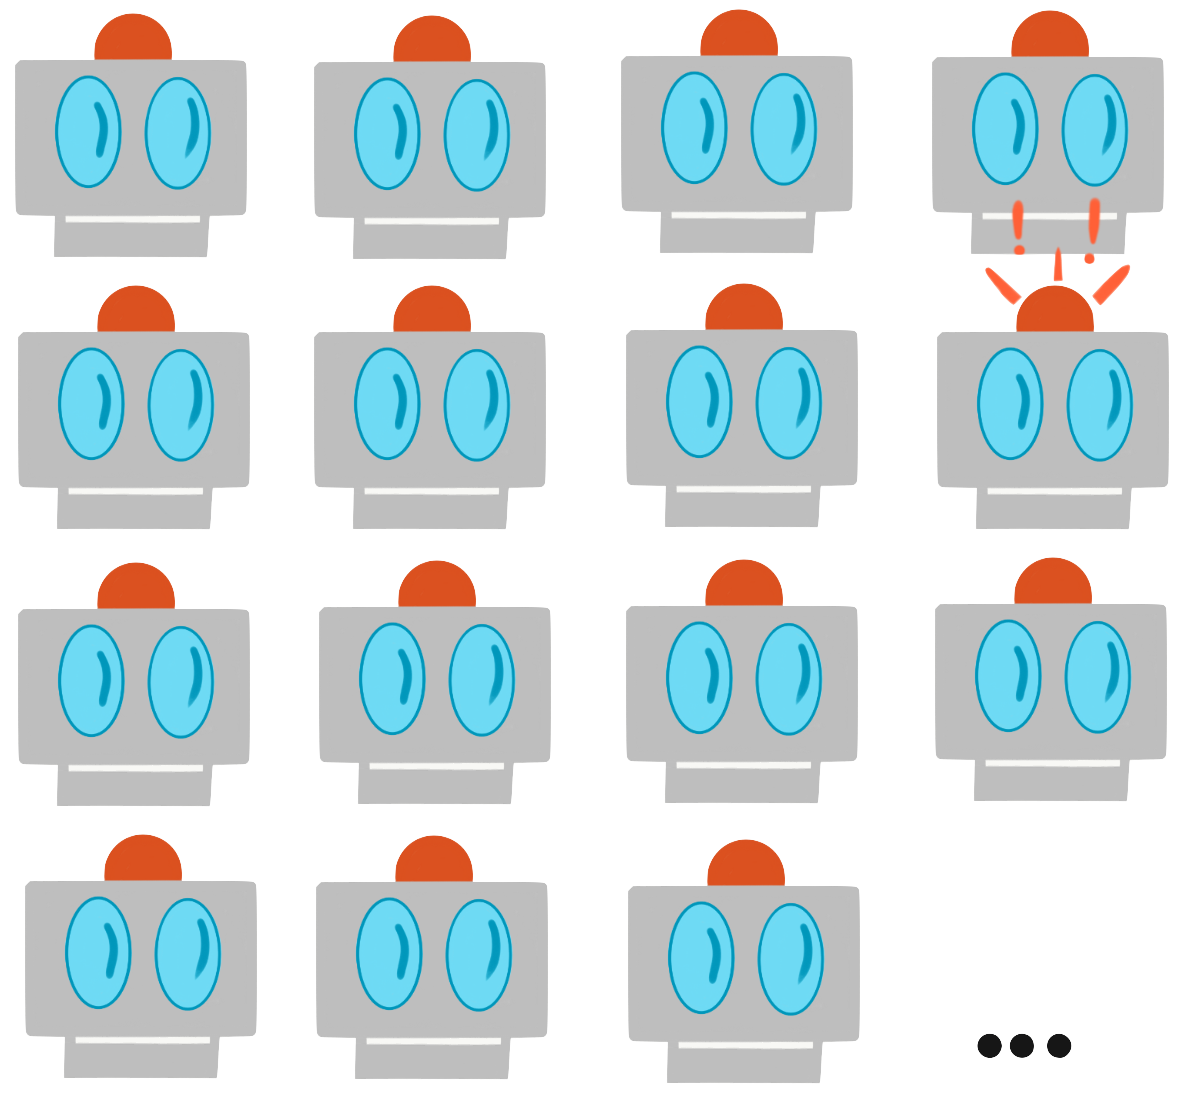
\includegraphics[width=0.9\textwidth]{img/dnn_collection}
   \end{column}
   \begin{column}{0.4\textwidth}
   
\includegraphics[width=0.9\textwidth]{img/cat}
   \end{column}
	\end{columns}
\captionsetup{singlelinecheck=off,justification=raggedright}
  	\caption{Several hundred fitness niches are defined using DNNs each trained to recognize different categories \cite{Nguyen2015InnovationLearning}.}
    \label{fig:niches}
\end{figure}
\end{frame}

\begin{frame}{Promoting Evolvability: Fitness Niches}
\vspace{2ex}	
\begin{figure}
    \centering
    \begin{columns}
    \begin{column}{0.7\textwidth}
     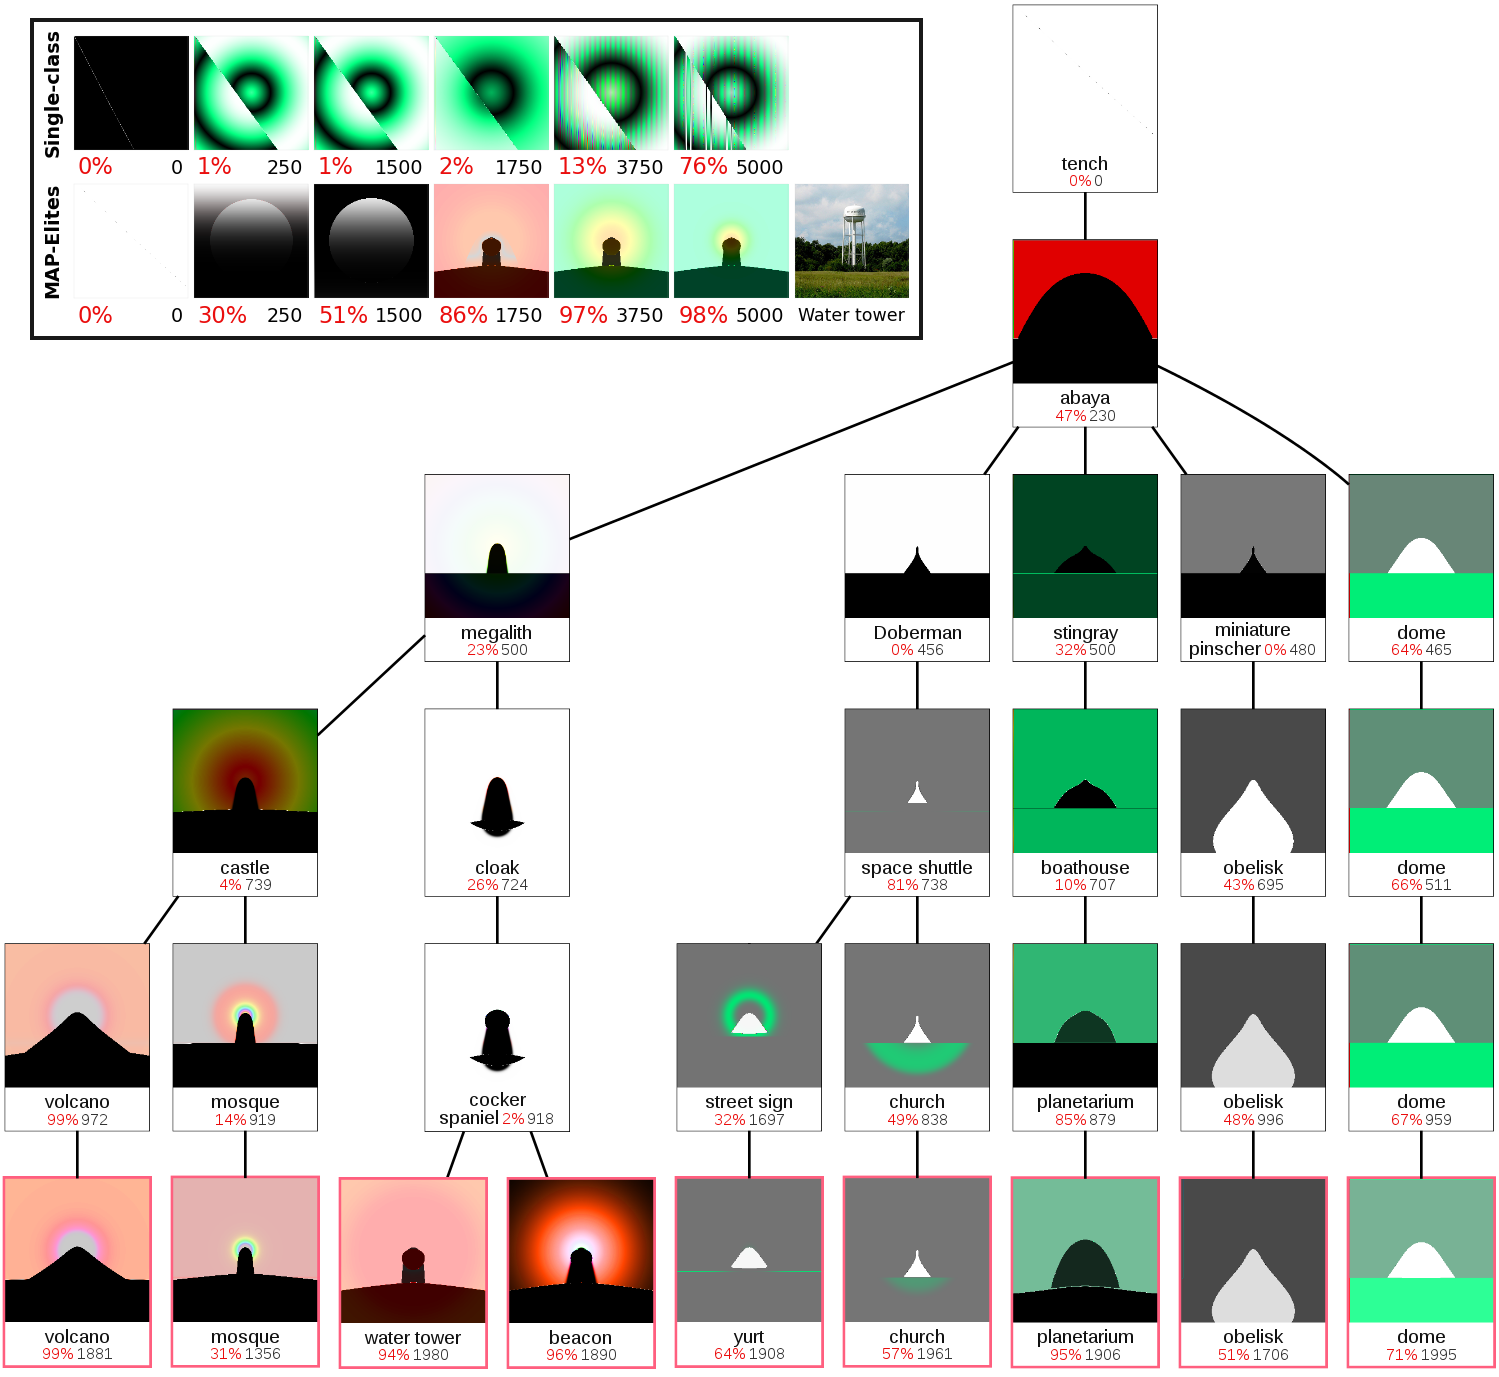
\includegraphics[width=\textwidth]{img/ie_phylogenetic_tree_combined}
    \end{column}
    \begin{column}{0.3\textwidth}
   	\captionsetup{singlelinecheck=off,justification=raggedright}
  	\caption{An illustration of goal-switching, where offspring from a parent that occupies one niche invade another \cite[Figure 9]{Nguyen2015InnovationLearning}. Individuals that promote phenotypically variable offspring are rewarded \cite{Mengistu2016EvolvabilityIt}.}
    \label{fig:goal_switching}
    \end{column}
    \end{columns}
   

\end{figure}
\end{frame}

\begin{frame}{Promoting Evolvability: Fitness Niches}
	\begin{figure}
    \centering
    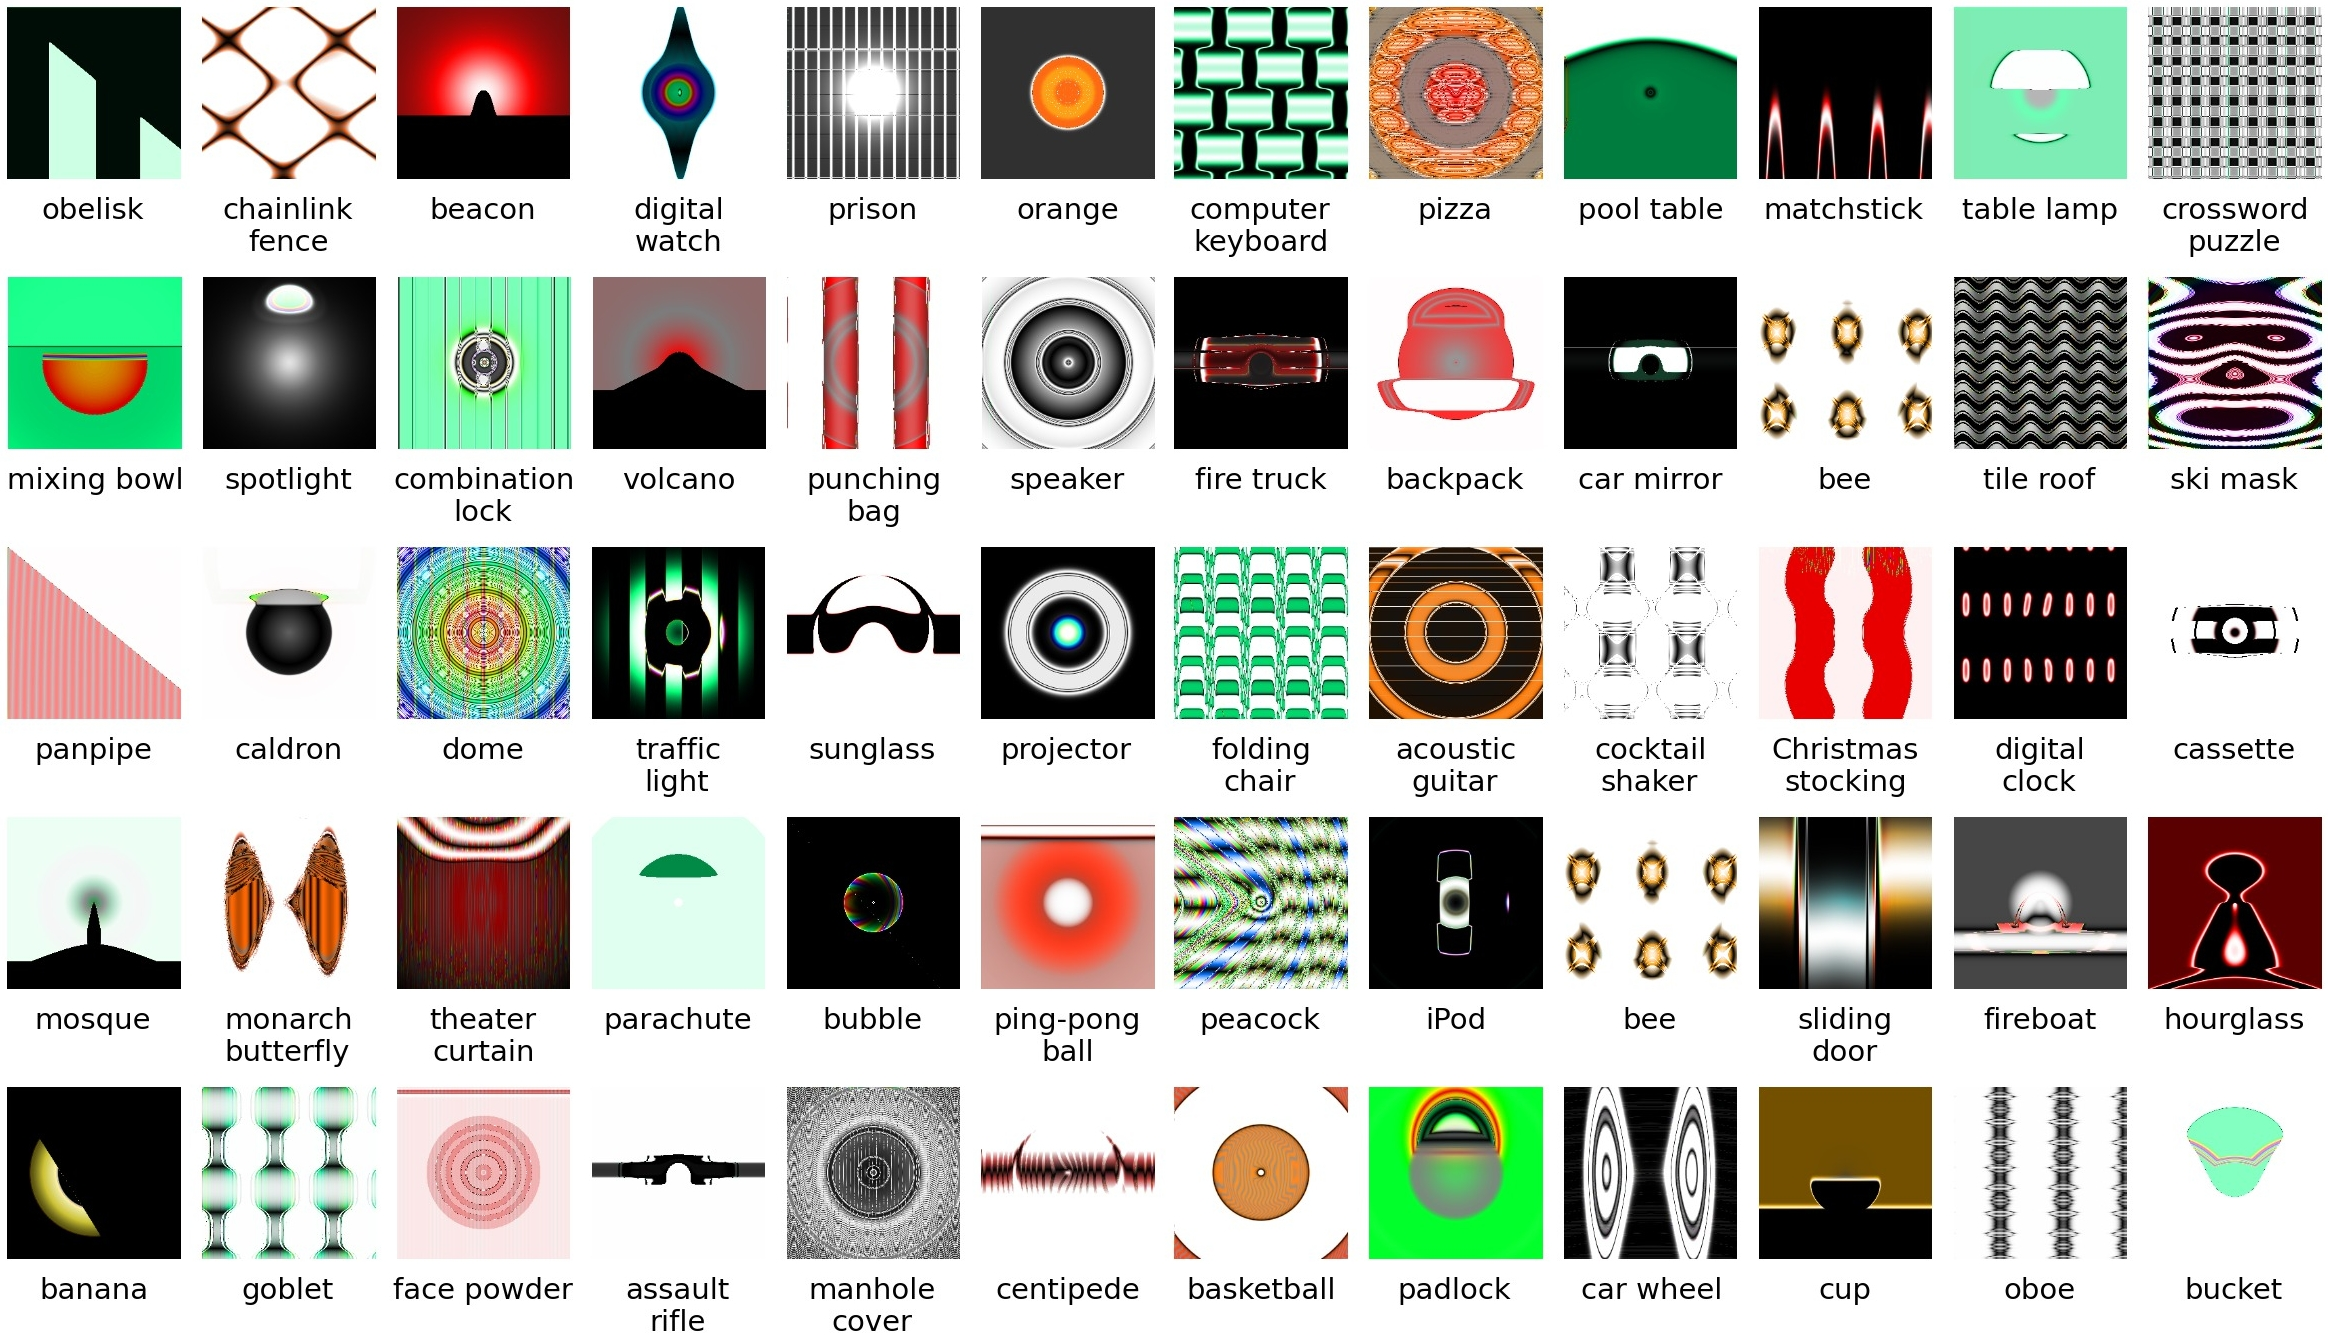
\includegraphics[width=0.9\textwidth]{img/ie_greatest_hits}
 	\captionsetup{singlelinecheck=off,justification=raggedright}
  	\caption{Selected champion individuals from a sample of environmental niches \cite[Figure 7]{Nguyen2015InnovationLearning}.}
    \label{fig:ie_results}
\end{figure}
\end{frame}
